\documentclass[sigconf]{acmart}

\usepackage{booktabs} % For formal tables
\usepackage{blindtext} % Package to generate dummy text throughout this template 
\usepackage{lettrine} % The lettrine is the first enlarged letter at the beginning of the text

% Pacotes de Gráficos
\usepackage{tikz} \usetikzlibrary{calc,plotmarks}  
\usepackage{pgfplots}
\usepackage{graphicx}

% Copyright
%\setcopyright{none}
%\setcopyright{acmcopyright}
%\setcopyright{acmlicensed}
\setcopyright{rightsretained}
%\setcopyright{usgov}
%\setcopyright{usgovmixed}
%\setcopyright{cagov}
%\setcopyright{cagovmixed}


% DOI
\acmDOI{10.475/123_4}

% ISBN
\acmISBN{123-4567-24-567/08/06}

%Conference
\acmConference[SBES'17]{SBES 2017: 31st Brazilian Symposium on Software Engineering}{Setembro 2017}{Fortaleza, Cear\'a Brasil} 
\acmYear{2017}
\copyrightyear{2017}

\acmPrice{15.00}


\begin{document}
\title{Cheiros de C\'odigo em projetos Android. Um estudo qualitativo sobre a percep\c{c}\~ao de desenvolvedores}
% \titlenote{Produces the permission block, and copyright information}
% \subtitle{Extended Abstract}
% \subtitlenote{The full version of the author's guide is available as
%   \texttt{acmart.pdf} document}


\author{Suelen G. Carvalho}
% \authornote{Dr.~Trovato insisted his name be first.}
% \orcid{1234-5678-9012}
\affiliation{
  \institution{Universidade de S\~ao Paulo}
  \streetaddress{Rua do Mat\~ao, 1010}
  \city{São Paulo} 
  \state{SP} 
  \postcode{05508-090}
}
\email{suelengc@ime.usp.br}

\author{Marco Aur\'elio Gerosa}
\affiliation{
  \institution{Universidade de S\~ao Paulo}
  \streetaddress{Rua do Mat\~ao, 1010}
  \city{S\~ao Paulo} 
  \state{SP} 
  \postcode{05508-090}
}
\email{gerosa@ime.usp.br}

\author{Maur\'icio Aniche}
\affiliation{
  \institution{Delft University of Technology}
  \streetaddress{Mekelweg 2}
  \city{Delft} 
  \state{Netherland} 
  \postcode{2628}
}
\email{m.f.aniche@tudelft.nl}

% The default list of authors is too long for headers}
\renewcommand{\shortauthors}{B. Trovato et al.}


\begin{abstract}
Android is the most widely used mobile operating system with 83\% of the world market and more than 2 million applications available in the official store. Android applications have been made complex software projects that need to be quickly developed and regularly evolved to meet the requirements of users. This context can lead to bad code design choices, known as code smells, that can become anomalies that degrade project quality, making it difficult to maintain. Consequently, software developers need to identify problematic code snippets in order to have a code base that favors maintenance and evolution. For this, developers often make use of techniques to detect code smells. Although there are already several code smells cataloged, such as God Class and Long Method, they do not take into account the nature of the project. Researches demonstrated that different platforms, languages and frameworks present specific code quality metrics. Android projects have specific characteristics, such as a directory that stores all the resources used and a class that tends to accumulate various responsibilities. Research on Android are still few. In this dissertation we aim to identify, validate and document code smells related with presentation layer of Android, where the greatest differences are found when compared to traditional projects. In other works on Android, were identified code smells related to safety, intelligent features or somehow impact the experience or user expectation consumption. Unlike them, our proposal is to catalog code smells Android that influence the quality of the code. With this, developers will have another resource for producing quality code.

\noindent \textbf{Keywords:} android, code smells, code quality, code anomalies, code metrics.
\end{abstract}

%
% The code below should be generated by the tool at
% http://dl.acm.org/ccs.cfm
% Please copy and paste the code instead of the example below. 
%
\begin{CCSXML}
<ccs2012>
 <concept>
  <concept_id>10010520.10010553.10010562</concept_id>
  <concept_desc>Computer systems organization~Embedded systems</concept_desc>
  <concept_significance>500</concept_significance>
 </concept>
 <concept>
  <concept_id>10010520.10010575.10010755</concept_id>
  <concept_desc>Computer systems organization~Redundancy</concept_desc>
  <concept_significance>300</concept_significance>
 </concept>
 <concept>
  <concept_id>10010520.10010553.10010554</concept_id>
  <concept_desc>Computer systems organization~Robotics</concept_desc>
  <concept_significance>100</concept_significance>
 </concept>
 <concept>
  <concept_id>10003033.10003083.10003095</concept_id>
  <concept_desc>Networks~Network reliability</concept_desc>
  <concept_significance>100</concept_significance>
 </concept>
</ccs2012>  
\end{CCSXML}

% \ccsdesc[500]{Computer systems organization~Embedded systems}
% \ccsdesc[300]{Computer systems organization~Redundancy}
% \ccsdesc{Computer systems organization~Robotics}
% \ccsdesc[100]{Networks~Network reliability}

% We no longer use \terms command
%\terms{Theory}

\keywords{android, cheiros de c\'odigo, qualidade de c\'odigo}


\maketitle

\section{Introdu\c{c}\~ao}
% -*- root: article.tex -*-
% \lettrine[nindent=0em,lines=3]{L}orem ipsim ult as 
Escrever código com qualidade tem se tornado cada vez mais importante com o aumento da complexidade de tecnologias e anseio dos usuários por novas funcionalidade e atualizações \cite{Hecht2015,MobileSmells:13}. Existem diferentes práticas, padrões e ferramentas que auxiliam os desenvolvedores a escrever código com qualidade, incluindo \textit{design patterns} \cite{gof} e cheiros de código \cite{Refactoring:99}. A falta de qualidade resulta em defeitos de software que custam a empresas quantias significativas, especialmente quando conduzem a falhas de software \cite{Nagappan:2005, briand1993modeling}. Evolução e manutenção de software também já se provaram como os maiores gastos com aplicações \cite{RefactoringAndImprovements:10}.

Uma das formas de aumentar a qualidade de software é identificar trechos de códigos ruins e refatorá-los, ou seja, alterar o código sem alterar o comportamento \cite{Refactoring:99}. Desta forma, temos que cheiros de código são aliados importantes na busca por qualidade de código pois, representam sintomas que podem indicar problemas mais profundos no software, não necessariamente, sendo o problema em si \cite{CodeSmell:06}. Seu mapeamento possibilita a definição de heurísticas que, por sua vez, possibilitam a implementação de ferramentas que os identificam de modo automático no código. PMD \cite{PMD2016}, Checkstyle e FindBugs são exemplos de ferramentas que identificam automaticamente alguns tipos de cheiros de código em projetos Java. 

Enquanto que cheiros de código em projetos Java já foram extensivamente estudados \cite{Riel, Refactoring:99, Martin:2008:CCH:1388398}, ainda há muito a se pesquisar sobre cheiros de código em projetos Android. No entanto, determinar o que é ou não um cheiro de código é subjetivo e pode variar de acordo com a tecnologia, desenvolvedor, metodologia de desenvolvimento dentre outros aspectos \cite{WikiCodeSmell}. Em particular, Aniche et al. \cite{MvcSmells:16,aniche2016satt} mostraram que a arquitetura do software é um fator importante e que deve ser levada em conta ao analisar a qualidade de um sistema. Outros estudos identificaram cheiros de código específicos Android relacionados ao consumo inteligente de recursos do dispositivo, como bateria e memória, usabilidade, dentre outros \cite{EnergyAndroidSmells, ReimannBrylski2013}. Verloop \cite{MobileSmells:13} analisou se classes derivadas do SDK Android são mais ou menos propensas a cheiros de código tradicionais do que classes puramente Java. Linares et al. \cite{DomainMatters} usaram o método DECOR para realizar a detecção de 18 \textit{anti-patterns} orientado a objetos em aplicativos móveis.

% Umme et al. \cite{Mannan_Dig_Ahmed_Jensen_Abdullah_Almurshed} recentemente levantaram que, das principais conferências de manutenção de software (ICSE, FSE, OOPSLA/SPLASH, ASE, ICSM/ICSME, MRS e ESEM), dentre 2008 a 2015, apenas 10\% dos artigos consideraram em suas pesquisas, projetos Android. Nenhuma outra plataforma móvel foi considerada.  

Nossa pesquisa complementa as anteriores no sentido de que também buscamos por cheiros de código Android. E se difere delas pois buscamos cheiros de código relacionados à qualidade, em termos de manutenabilidade e legibilidade, específico dessa plataforma. Por exemplo \textsc{Activities}, \textsc{Fragments} e \textsc{Adapters} são classes usadas na construção de telas e \textsc{listeners} são responsáveis pelas interações com os usuários. Buscamos entender então quais são as \emph{boas e más} práticas no desenvolvimento da interface visual Android. 

% Para limitar nosso objeto de estudo, optamos por focar em cheiros de código relacionados ao \textit{front-end} Android pois encontramos pesquisas com abordagem similar, porém relacionadas ao \textit{front-end} de tecnologias web, como CSS \cite{CSSCodeSmell}, Javascript \cite{BB} e o arcabouço Spring MVC \cite{FinavaroAniche2016}. 

% E enquanto que cheiros de código em projetos Java já foram extensivamente estudados \cite{Riel, Refactoring:99, Martin:2008:CCH:1388398}, o \textit{front-end} Android ainda carece de estudo e possui peculiaridades não encontradas em código Java tradicional \cite{Mannan_Dig_Ahmed_Jensen_Abdullah_Almurshed}. Alguns exemplos dessas peculiaridas são o ciclo de vida de \textsc{Activities} e \textsc{Fragments} e a criação da interface visual que é feita através de arquivos XML chamados de \textsc{layout resources}.
 

Por meio de um questionário online com perguntas sobre boas e más práticas relacionadas ao \textit{front-end} Android respondido por 45 desenvolvedores, derivamos 23 más práticas. Validamos a percepção dos desenvolvedores sobre essas más práticas através de um experimento com outros 20 desenvolvedores. Os resultados mostram que de fato existem boas e más práticas específicas ao \textit{front-end} Android. Ainda que tenhamos validado com sucesso a percepção dos desenvolvedores sobre apenas duas, esperamos que este catálogo de más práticas possa contribuir com ideias iniciais para outras pesquisas sobre qualidade de codigo em projetos Android.

 % para a definição de cheiros de código e heurísticas para a detecção sistematizada das mesmas em projetos Android, além de contribuir com sugestões de como mitigá-las.

As contribuições deste trabalho são:

\begin{enumerate}

	\item Catálogo com 23 más práticas e sugestões de soluções no desenvolvimento do \textit{front-end} Android, derivadas a partir dos resultados obtidos com a aplicação de um questionário online respondido por 45 desenvolvedores.

	\item A percepção de desenvolvedores sobre as quatro más práticas de alta recorrência através de um questionário online com 20 desenvolvedores. Sendo que obtivemos um resultado positivo e estatísticamente válido sobre duas delas.

	\item Apêndice online~\cite{apendice} com roteiros dos questionários e outras informações da pesquisa para que outros pesquisadores possam replicar nosso estudo.

\end{enumerate}


% \begin{enumerate}
% 	\item Catálogo com 23 más práticas no desenvolvimento do \textit{front-end} Android, derivadas a partir dos resultados obtidos com a aplicação de um questionário online respondido por 45 desenvolvedores.
% 	\item A percepção de desenvolvedores sobre as quatro más práticas mais recorrentes através de um questionário online com 11 desenvolvedores..
% 	\item Apêndice online \footnote{Apêndice online: http://suelengc.com/android-code-smells-article} com roteiros dos quetionários e outras informações da pesquisa para que outros pesquisadores possam replicar nosso estudo.
% \end{enumerate}

As seções seguintes deste artigo estão organizadas da seguinte forma: a Seção \ref{metodologia} aborda a metodologia de pesquisa. A Seção \ref{resultados} apresenta o catálogo de más práticas a percepção de desenvovledores sobre as quatro mais recorrêntes. A Seção \ref{ameacas} aborda as ameaças à validade do estudo. A Seção \ref{relacionados} discute os trabalhos relacionados e o estado da arte sobre Android e cheiros de código. E por fim, a Seção \ref{conclusao} conclui.


\section{Trabalhos Relacionados}
% -*- root: article.tex -*-
Muitas pesquisas t\^em sido realizadas sobre a plataforma Android, muitas delas focam em vulnerabilidades \cite{Y, F, G, X, P, D, E}, autentica\c{c}\~ao \cite{T, Yamashita6405287, R} e testes \cite{J, M}. Diferentemente dessas pesquisas, nossa pesquisa tem foco na percep\c{c}\~ao dos desenvolvedores sobre boas e m\'as pr\'aicas de desenvolvimento na plataforma Android. 

A percep\c{c}\~ao desempenha um importante papel na defini\c{c}\~ao de code smells relacionados a uma tecnologia, visto que code smells possuem uma natureza subjetiva. Code smells desempenham um importante papel na busca por qualidade de c\'odigo, visto que, ap\'os mapeados, podemos chegar a heur\'isticas para identific\'a-los e com essas heur\'isticas, implementar ferramentas que automatizem o processo de identificar c\'odigos problem\'aticos.

Verloop \cite{MobileSmells:13} conduziu um estudo no qual avaliou por meio de 4 ferramentas de detec\c{c}\~ao automatizada de cheiros de c\'odigo (JDeodorant, Checkstyle, PMD e UCDetector) a presen\c{c}a de 5 cheiros de c\'odigo (Long Method, Large Class, Long Parameter List, Feature Envy e Dead Code) em 4 projetos Android. Nossa pesquisa se relaciona com a de Verloop no sentido de que tamb\'em estamos buscando por cheiros de c\'odigo, entretanto, em vez de de buscarmos por cheiros de c\'odigo j\'a definidos, realizamos uma abordagem inversa na qual, primeiro buscamos entender a percep\c{c}\~ao de desenvolvedores sobre boas e m\'as pr\'aticas em Android, e a partir dessa percep\c{c}\~ao, relacionamos com algum cheiro de c\'odigo pr\'e-existente ou derivamos algum novo.

Gottschalk et al \cite{EnergyAndroidSmells} conduziram um estudo sobre formas de detectar e refatorar cheiros de c\'odigo relacionados ao uso efici\^ente de energia. Os autores compilaram um cat\'alogo com 8 cheiros de c\'odigo e trabalharam sob um trecho de c\'odigo Android para exemplificar um deles, o "binding resource too early", quando algum recurso \'e alocado muito antes de precisar ser utilizado. Essa pesquisa \'e relacionada \`a nossa por ambas considerarem a tecnologia Android e se diferenciam pois focamos na busca por cheiros de c\'odigo relacionados a qualidade de c\'odigo, no sentido de legibilidade e manutenablidade.

Aplicativos Android s\~ao escritos na linguagem de programa\c{c}\~ao Java \cite{AndroidFundamentals}. Ent\~ao a primeira quest\~ao \'e: por que buscar por \textit{smells} Android sendo que j\'a existem tantos \textit{smells} Java? Pesquisas t\^em demonstrado que tecnologias diferentes podem apresentar \textit{code smells} espec\'ificos, como por exemplo Aniche et al. identificaram 6 \textit{code smells} espec\'ificos ao framework Spring MVC, um framework Java para desenvolvimento web. Outras pesquisas concluem que projetos Android possuem caracter\'isticas diferentes de projetos java \cite{Hecht2015, Mannan_Dig_Ahmed_Jensen_Abdullah_Almurshed, ReimannBrylski2013}, por exemplo, o \textit{front-end} \'e representado por arquivos XML e o ponto de entrada da aplica\c{c}\~ao \'e dado por \textit{event-handler} \cite{AndroidActivities2016} como o m\'etodo \textsc{onCreate}. Encontramos tamb\'em diversas pesquisas sobre \textit{code smells} sobre tecnologias usadas no desenvolvimento de \textit{front-end} web como CSS \cite{CSSCodeSmell} e JavaScript \cite{BB}. Essas pesquisas nos inspiraram a buscar entender se existem \textit{code smells} no \textit{front-end} Android. \\


% \textbf{[se\c{c}\~ao n\~ao finalizada, \'a concluir.]}

\section{Metodologia}
% -*- root: article.tex -*-
Durante o processo de codificação das respostas para as 18 perguntas abertas sobre boas e m\'as pr\'aticas, 	
Conduzimos um estudo qualitativo e explorat\'orio onde os dados foram coletados atrav\'es de um question\'ario online com desenvoveldores Android. Esta se\c{c}\~ao descreve de forma detalhada a estrutura do question\'ario, os participantes e a an\'alise realizada sobre as respostas obtidas.

\subsection{Question\'ario}
\label{sub:questionario}

O question\'ario continha 25 quest\~oes divididas em tr\^es se\c{c}\~oes: a primeira se\c{c}\~ao continha 6 perguntas demogr\'aficas, a segunda se\c{c}\~ao continha 16 perguntas sobre boas e m\'as pr\'aticas relacionadas ao \textit{front-end} Android e a terceira se\c{c}\~ao continha 3 perguntas, 2 para obter \'ultimos pensamentos sobre boas e m\'as pr\'aticas e 1 solicitando email caso o participante tivesse interesse em etapas futuras da pesquisa. O question\'ario foi escrito em ingl\^es por\'em informava o participante que respostas em ingl\^es ou portugu\^es eram aceitas. Antes da divulga\c{c}\~ao, realizamos um piloto com 3 desenvolvedores Android. Todos estes dados est\~ao dispon\'iveis no nosso pacote de replica\c{c}\~ao\footnote{https://github.com/SuelenGC/android-code-smells-article}.

A primeira se\c{c}\~ao continha 6 quest\~oes demogr\'aficas obrigat\'orias de multipla escolha. Abordavam sobre idade (18 ou menos, 19 a 24, 25 a 34 e assim por diante at\'e 55 ou mais), estado de resid\^encia (foi dada uma lista com estados do Brasil, Estados Unidos e Europa), anos de experi\^encia com desenvolvimento de software, (1 anos ou menos, 2 anos, 3 anos, e assim por diante at\'e 10 ou mais), anos de experi\^encia com desenvolvimento Android (mesma escala de anos da quest\~ao anterior), uma quest\~ao sobre linguagens que o participante se considerava proeficiente (Java, Python, Ruby, Android, dentre outras) e sobre o \'ultimo grau de escolaridade (estudante de bacharelado, bacharelado, mestrado e doutorado). As quest\~oes sobre idade, regi\~ao, linguagens e grau de escolaridade continham a op\c{c}\~ao ``outros'' para o caso de nenhuma das outras op\c{c}\~oes atenderem, ao selecionar ``outros'' era poss\'ivel escrever uma resposta de forma manual.

A segunda se\c{c}\~ao continha 16 quest\~oes opcionais e dissertativas sobre boas e m\'as pr\'aticas relacionadas ao \textit{front-end} Android. Para cada elemento do \textit{front-end} Android foram feitas duas perguntas, uma sobre boas e outra sobre m\'as pr\'aticas percebidas pelos participantes. Por exemplo, para o elemento \textsc{Activity} foram feitas as perguntas:

\begin{itemize} 
	\item[$\textasteriskcentered$] Do you have any good practices to deal with Activities?
	\item[$\textasteriskcentered$] Do you have any bad practices to deal with Activities? 
\end{itemize}

A terceira se\c{c}\~ao continha 3 perguntas opcionais e dissertativas, 2 para captar qualquer \'ultima ideia sobre boas e m\'as pr\'aticas n\~ao captadas nas quest\~oes anteriores e 1 solicitando o email do participante caso o mesmo tivesse interesse em participar de etapas futuras da pesquisa. As perguntas sobre boas e m\'as pr\'aticas foram as a seguir: 

\begin{itemize} 
	\item[$\textasteriskcentered$] Are there any other *GOOD* practices in Android Presentation Layer we did not asked you or you did not said yet?
	\item[$\textasteriskcentered$] Are there any other *BAD* practices in Android Presentation Layer we did not asked you or you did not said yet?
\end{itemize}

Antes da divulga\c{c}\~ao, realizamos um piloto com 3 desenvolvedores Android e com o feedback deles fizemos alguns ajustes relacionados a obrigatoriedade das perguntas da segunda se\c{c}\~ao do question\'ario, onde todas tornaram-se opcionais. As respostas dos participantes piloto foram desconsideradas para efeitos de vi\'es. 

\subsection{Participantes}
\label{sub:participantes}

O question\'ario foi divulgado em redes sociais como Facebook, Twitter e Linkedin, em grupos de discuss\~ao sobre Android como \href{https://groups.google.com/forum/#!forum/androidbrasil-dev}{\textit{Android Dev Brasil}}, \href{https://groups.google.com/forum/\#!forum/android-brasil-projetos}{\textit{Android Brasil Projetos}} e o grupo do \href{http://slack.androiddevbr.org/}{\textit{Slack Android Dev Br}}, maior grupo de desenvolvedores Android do Brasil com 2622 participantes at\'e o momento da escrita deste artigo. 

O question\'ario esteve aberto por aproximadamente 3 meses e meio, de 9 de Outubro de 2016 at\'e 18 de Janeiro de 2017. Recebemos um total de 45 respostas sendo que 41 foram submetidas em Outubro, 3 no come\c{c}o de Novembro e 1 em Janeiro. Uma poss\'ivel explica\c{c}\~ao para praticamente n\~ao termos tido respostas nos meses de Novembro e Dezembro pode ser as festas comemorativas de final de ano. 

80\% dos participantes responderam pelo menos 3 perguntas sobre boas e m\'as pr\'aticas no \textit{front-end} Android (7 responderam de 3 a 6, 6 responderam de 8 a 10 e 23 responderam 13 ou mais, sendo que desses, 14 responderam todas) e apenas 20\% responderam uma (2 participantes) ou nenhuma (7 participantes). A pergunta solicitando o email foi respondida por 53\% dos participantes, o que pode indicar um interesse leg\'itimo da comunidade de desenvolvedores Android pelo tema, refor\c{c}ando a relev\^ancia do estudo. A Tabela \ref{tab:ResponseRate} apresenta o percentual de respostas obtido por cada uma das 18 perguntas sobre boas e m\'as pr\'aticas, podemos notar que a menor taxa de respostas foi na quest\~ao 18 e a maior na quest\~ao 1.

\begin{table*}[t]
\centering
\caption{Percentual de respostas das perguntas sobre boas e m\'as pr\'aticas.}
\footnotesize
\begin{tabular}{lp{12cm}c}
\toprule
\multicolumn{2}{@{}l}{\textbf{Quest\~oes}} 	& 	\multicolumn{1}{c}{\textbf{Taxa de Respostas}} \\
\hline
\multicolumn{1}{@{}l}{Q1} & Do you have any good practices to deal with \textsc{Activities}?	& 	80 \% \\ 
\multicolumn{1}{@{}l}{Q2} & Do you have anything you consider a bad practice when dealing with \textsc{Activities}?	& 	78 \% \\ 
\multicolumn{1}{@{}l}{Q3} & Do you have any good practices to deal with \textsc{Fragments}?	& 	73 \% \\ 
\multicolumn{1}{@{}l}{Q4} & Do you have anything you consider a bad practice when dealing with \textsc{Fragments}?	& 	69 \% \\ 
\multicolumn{1}{@{}l}{Q5} & Do you have any good practices to deal with \textsc{Adapters}?	& 	67 \% \\ 
\multicolumn{1}{@{}l}{Q6} & Do you have anything you consider a bad practice when dealing with \textsc{Adapters}?	& 	60 \% \\ 
\multicolumn{1}{@{}l}{Q7} & Do you have any good practices to deal with \textsc{Listeners}?	& 	53 \% \\ 
\multicolumn{1}{@{}l}{Q8} & Do you have anything you consider a bad practice when dealing with \textsc{Listeners}?	& 	51 \% \\ 
\multicolumn{1}{@{}l}{Q9} & Do you have any good practices to deal with \textsc{Layout Resources}?	& 	62 \% \\ 
\multicolumn{1}{@{}l}{Q10} & Do you have anything you consider a bad practice when dealing with \textsc{Layout Resources}?	& 	51 \% \\ 
\multicolumn{1}{@{}l}{Q11} & Do you have any good practices to deal with \textsc{Styles Resources}?	& 	51 \% \\ 
\multicolumn{1}{@{}l}{Q12} & Do you have anything you consider a bad practice when dealing with \textsc{Styles Resources}?	& 	49 \% \\ 
\multicolumn{1}{@{}l}{Q13} & Do you have any good practices to deal with \textsc{String Resources}?	& 	62 \% \\ 
\multicolumn{1}{@{}l}{Q14} & Do you have anything you consider a bad practice when dealing with \textsc{String Resources}?	& 	51 \% \\ 
\multicolumn{1}{@{}l}{Q15} & Do you have any good practices to deal with \textsc{Drawable Resources}?	& 	53 \% \\ 
\multicolumn{1}{@{}l}{Q16} & Do you have anything you consider a bad practice when dealing with \textsc{Drawable Resources}?	& 	47 \% \\ 
\multicolumn{1}{@{}l}{Q17} & Are there any other *GOOD* practices in Android Presentation Layer we did not asked you or you did not said yet?	& 	49 \% \\ 
\multicolumn{1}{@{}l}{Q18} & Are there any other *BAD* practices in Android Presentation Layer we did not asked you or you did not said yet?	& 	44 \% \\ 
\toprule
\end{tabular}
\label{tab:ResponseRate}
\end{table*}

Com a an\'alise das quest\~oes demogr\'aficas foi poss\'ivel notar que atingimos com sucesso \textit{desenvolvedores Android com variados n\'iveis de experi\^encia e de diversas regi\~oes} pois: 1) 100\% dos participantes indicaram possuir alguma experi\^encia com desenvolvimento Android, 2) menos de 14\% indicaram possuir 1 anos ou menos de experi\^encia com Android e mais de 86\% indicaram 2 anos ou mais (15,5\% 2 anos, 13,3\% 4 anos, 6,5\% 5 anos, 15,5\% 6 anos, 4,4\% 7 anos e 4,4\% 8 anos), 4) 36 respostas foram do Brasil, 7 de pa\'ises europeus e 1 dos Estados Unidos (Calif\'ornia). Vale lembrar que a plarforma Android completa 10 anos em 2017, ou seja, 5 anos de experi\^encia nessa plataforma representa 50\% do tempo de vida dela desde seu an\'uncio em 2007. Esses dados, sobre a experi\^encia dos participantes, s\~ao apresentados na Tabela \ref{tab:DadosDemograficos}.

\begin{table}[h]
\centering
\caption{Experi\^encia dos participantes com desenvolvimento Android.}
\small
\begin{tabular}{l|c|r}
\toprule
\textbf{Anos de Experi\^encia} & \textbf{Participantes} & \multicolumn{1}{c}{\textbf{\%}}  \\
\hline
1 ano ou menos 	&	 6 		& 	13,3 \%	 \\
2 anos 			& 	 7 		& 	15,6 \%	 \\
3 anos 			& 	 12		& 	26,7 \%	 \\
4 anos 			& 	 6 		& 	13,3 \%	 \\
5 anos 			& 	 3 		& 	 6,7 \%	 \\
6 anos 			& 	 7 		& 	15,6 \%	 \\
7 anos 			& 	 2 		& 	 4,4 \%	 \\
8 anos 			& 	 2 		& 	 4,4 \%	 \\
\toprule
\end{tabular}
\label{tab:DadosDemograficos}
\end{table}

% \begin{tikzpicture}
% \begin{axis}[
%     ybar,
%     enlargelimits=0.15,
%     legend style={at={(0.5,-0.15)},
%       anchor=north,legend columns=-1},
%     ylabel={participantes},
%     symbolic x coords={1-2 anos,2-5 anos,6-10 anos},
%     xtick=data,
%     nodes near coords,
%     nodes near coords align={vertical},
%     ]
% \addplot coordinates {(1-2 anos,5) (2-5 anos,10) (6-10 anos,30)};
% \addplot coordinates {(1-2 anos,13) (2-5 anos,21) (6-10 anos,11)};
% \legend{experi\^encia com software,experi\^encia com Android}
% \end{axis}
% \end{tikzpicture}

\subsection{An\'alise dos Dados}
\label{sub:smells-definition}

O processo de an\'alise partiu da listagem das 45 respostas do question\'ario e se deu em 5 passos: verticaliza\c{c}\~ao, limpeza dos dados, codifica\c{c}\~ao, divis\~ao e agrupamento das categorias. 

O processo que denominamos de \textit{verticaliza\c{c}\~ao} consistiu em considerar cada resposta de boa ou m\'a pr\'atica como um registro individual a ser analisado. Ou seja, cada participante respondeu 18 perguntas sobre boas e m\'as pr\'aticas no \textit{front-end} Android (2 perguntas para cada elemento e mais duas perguntas gen\'ericas). Com o processo de \textit{verticaliza\c{c}\~ao}, cada uma dessas respostas se tornou um registro, ou seja, cada participante resultava em 18 respostas a serem analisadas, totalizando 810 respostas (18 perguntas multiplicado por 45 participantes) sobre boas e m\'as pr\'aticas.

O passo seguinte foi realizar a \textit{limpeza dos dados}. Esse passo consistiu em remover respostas obviamente n\~ao \'uteis como respostas em branco, que continham frases como \textit{"N\~ao"}, \textit{"N\~ao que eu saiba"}, \textit{"Eu n\~ao me lembro"} e similares, as consideradas vagas como \textit{"Eu n\~ao tenho certeza se s\~ao boas praticas mas uso o que vejo por ai"}, as consideradas gen\'ericas como \textit{"Como todo c\'odigo java..."} e as que n\~ao eram relacionadas a boas pr\'aticas de c\'odigo. Das 810 boas e m\'as pr\'aticas, 352 foram consideradas e 458 desconsideradas. Das 352, 44,6\% foram apontadas como m\'as pr\'aticas e 55,4\% como boas pr\'aticas. 

Em seguida, realizamos a codifica\c{c}\~ao sobre as boas e m\'as pr\'aticas. O processo de codifica\c{c}\~ao consistiu em analisar cada resposta e atribuir uma ou mais categorias. Durante esse processo, houveram 30 respostas que n\~ao eram triviais de identificar uma categoria ou mesmo de dizer se essas respostas deveriam ser consideradas. Essas respostas foram marcadas como \textit{"talvez"} e reavaliadas ao final, onde 6 permaneceram e 24 foram desconsideradas. Ainda durante a codifica\c{c}\~ao, 9 respostas incialmente consideradas, foram desconsideradas. Para toda resposta desconsiderada nesse passo, foi indicado um motivo. Ao final da codifica\c{c}\~ao, as categorias foram agrupadas por temas.

Por \'ultimo realizamos o passo de divis\~ao. Esse passo consistiu em dividir as respostas que receberam mais de uma categoria em duas ou mais respostas, de acordo com o n\'umero de categorias identificadas, de forma a resultar em uma categoria por resposta. Por exemplo, a resposta \textit{"N\~ao fazer Activities serem callbacks de execu\c{c}\~oes ass\'incronas. Herdar sempre das classes fornecidas pelas bibliotecas de suporte, nunca diretamente da plataforma"} indica na primeira ora\c{c}\~ao uma categoria e na segunda ora\c{c}\~ao, outra categoria. Ao divid\'i-la, mantivemos apenas o trecho da resposta relativo a categoria, como se fossem duas respostas distintas e v\'alidas. Em algumas divis\~oes realizadas, a resposta completa era necess\'aria para entender ambas as categoriza\c{c}\~oes, nesses casos, mantivemos a resposta original, mesmo que duplicada, e categorizamos cada uma de forma diferente. 

Ao final da an\'alise constavam 389 respostas individualmente categorizadas sobre boas e m\'as pr\'aticas no \textit{front-end} Android.

\section{Resultados}
% -*- root: article.tex -*-
Durante o processo de codifica\c{c}\~ao das 18 perguntas sobre boas e m\'as pr\'aticas, 56 categorias emergiram. Classificamos as categorias de acordo com sua recorr\^encia, ou seja, a quantidade de respostas a qual ela foi atribu\'ida. Utilizamos a seguinte escala: baix\'issima recorr\^encia significa menos de 3 respostas, baixa recorr\^encia significa de 3 a 7 respostas, m\'edia recorr\^encia significa de 8 a 20 respostas e alta recorr\^encia significa acima de 20 respostas.

Na Figura \ref{fig:CategoriaXRecorrencia} \'e poss\'ivel observar que o maior conjunto de categorias \'e o de baix\'issima recorr\^encia, ou seja, pouqu\'issimos participantes comentaram sobre esses assuntos. Em seguida, temos o conjunto de m\'edia, baixa e alta recorr\^encia, respectivamente.

\begin{figure}[!htb]
	\centering
	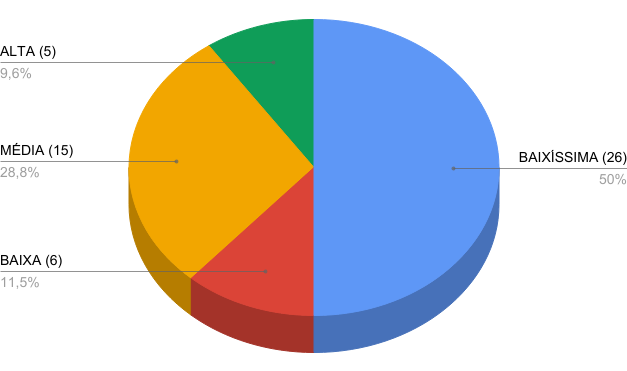
\includegraphics[width=0.45\textwidth]{grafico-recorrencia.png}
	\caption{Distribui\c{c}\~ao das Categorias x Recorr\^encia}
	\label{fig:CategoriaXRecorrencia}
\end{figure}


A Tabela \ref{tab:Categories} apresenta o n\'umero de ocorr\^encias das categorias de alta, m\'edia e baixa recorr\^encia em cada quest\~ao relacionada a boas e m\'as pr\'aticas. A \'ultima linha da tabela, \#Categorias, apresenta quantas categorias emergiram de cada quest\~ao, como cada quest\~ao est\'a diretamente ligada a um elemento do \textit{front-end} Android, podemos interpret\'a-la da seguinte forma: \textbf{quais s\~ao os pontos de aten\c{c}\~ao a serem analisados em determinado elemento Android?} A \'ultima coluna da tabela, \#Q, apresenta em quantas quest\~oes cada categoria surgiu, podemos interpret\'a-la da seguinte forma: \textbf{com base na categoria, quais elementos devem ser investigados}?

% Quando se criam categoriza\c{c}\~oes para auxiliar desenvolvedores a identificar pontos de aten\c{c}\~ao a serem avaliados e onde este pontos devem ser investigados especificamente no c\'odigo, pensando em qualidade de c\'odigo d\'a-se o nome de \textit{smells}. Portanto, nesta se\c{c}\~ao iremos compilar este conjunto de Android \textit{code smells} que identificamos atrav\'es das categoriza\c{c}\~oes.


\begin{table*}[t]
\centering
\footnotesize
\begin{tabular}{@{}p{3.8cm}p{0.3cm}p{.2cm}p{.2cm}p{.2cm}p{.2cm}p{.2cm}p{.2cm}p{.2cm}p{.2cm}p{.2cm}p{.4cm}p{.4cm}p{.4cm}p{.4cm}p{.4cm}p{.4cm}p{.4cm}p{.4cm}p{.4cm}p{0.2cm}@{}}
\toprule
\textbf{Categoria} & \multicolumn{1}{c}{\textbf{\#T}} & Q1 & Q2 & Q3 & Q4 & Q5 & Q6 & Q7 & Q8 & Q9 & Q10 & Q11 & Q12 & Q13 & Q14 & Q15 & Q16 & Q17 & Q18 &  \multicolumn{1}{c}{\textbf{\#Q}} \\
\hline
\multicolumn{2}{c}{\scriptsize{\textbf{ALTA RECORR\^ENCIA}}} \\
L\'ogica em Views							& \multicolumn{1}{c}{53} 	& \multicolumn{1}{c}{12} 	& \multicolumn{1}{c}{15} 	& \multicolumn{1}{c}{6} 	& \multicolumn{1}{c}{8} 	& \multicolumn{1}{c}{3} 	& \multicolumn{1}{c}{8} 	& \multicolumn{1}{c}{--} 	& \multicolumn{1}{c}{1} 	& \multicolumn{1}{c}{--} 	& \multicolumn{1}{c}{--} 	& \multicolumn{1}{c}{--} 	& \multicolumn{1}{c}{--} 	& \multicolumn{1}{c}{--} 	& \multicolumn{1}{c}{--} 	& \multicolumn{1}{c}{--} 	& \multicolumn{1}{c}{--} 	& \multicolumn{1}{c}{--} 	& \multicolumn{1}{c}{--} 	& \multicolumn{1}{c}{7} \\	
Padr\~ao de Nome de Recursos				& \multicolumn{1}{c}{24} 	& \multicolumn{1}{c}{1} 	& \multicolumn{1}{c}{--} 	& \multicolumn{1}{c}{--} 	& \multicolumn{1}{c}{--} 	& \multicolumn{1}{c}{--} 	& \multicolumn{1}{c}{--} 	& \multicolumn{1}{c}{--} 	& \multicolumn{1}{c}{--} 	& \multicolumn{1}{c}{3} 	& \multicolumn{1}{c}{2} 	& \multicolumn{1}{c}{3} 	& \multicolumn{1}{c}{2} 	& \multicolumn{1}{c}{8} 	& \multicolumn{1}{c}{2} 	& \multicolumn{1}{c}{3} 	& \multicolumn{1}{c}{--} 	& \multicolumn{1}{c}{--} 	& \multicolumn{1}{c}{--} 	& \multicolumn{1}{c}{8} \\	
Recursos M\'agicos							& \multicolumn{1}{c}{23} 	& \multicolumn{1}{c}{--} 	& \multicolumn{1}{c}{--} 	& \multicolumn{1}{c}{--} 	& \multicolumn{1}{c}{--} 	& \multicolumn{1}{c}{--} 	& \multicolumn{1}{c}{--} 	& \multicolumn{1}{c}{--} 	& \multicolumn{1}{c}{--} 	& \multicolumn{1}{c}{4} 	& \multicolumn{1}{c}{2} 	& \multicolumn{1}{c}{1} 	& \multicolumn{1}{c}{1} 	& \multicolumn{1}{c}{9} 	& \multicolumn{1}{c}{6} 	& \multicolumn{1}{c}{--} 	& \multicolumn{1}{c}{--} 	& \multicolumn{1}{c}{--} 	& \multicolumn{1}{c}{--} 	& \multicolumn{1}{c}{6} \\	
Views Aninhados								& \multicolumn{1}{c}{21} 	& \multicolumn{1}{c}{--} 	& \multicolumn{1}{c}{--} 	& \multicolumn{1}{c}{--} 	& \multicolumn{1}{c}{--} 	& \multicolumn{1}{c}{1} 	& \multicolumn{1}{c}{--} 	& \multicolumn{1}{c}{--} 	& \multicolumn{1}{c}{--} 	& \multicolumn{1}{c}{9} 	& \multicolumn{1}{c}{9} 	& \multicolumn{1}{c}{--} 	& \multicolumn{1}{c}{--} 	& \multicolumn{1}{c}{--} 	& \multicolumn{1}{c}{--} 	& \multicolumn{1}{c}{--} 	& \multicolumn{1}{c}{--} 	& \multicolumn{1}{c}{1} 	& \multicolumn{1}{c}{1} 	& \multicolumn{1}{c}{5} \\	

\vspace{1sp} \\
\multicolumn{2}{@{}c}{\scriptsize{\textbf{M\'EDIA RECORR\^ENCIA}}} \\ 
Padr\~ao MVP								& \multicolumn{1}{c}{17} 	& \multicolumn{1}{c}{8} 	& \multicolumn{1}{c}{2} 	& \multicolumn{1}{c}{5} 	& \multicolumn{1}{c}{--} 	& \multicolumn{1}{c}{--} 	& \multicolumn{1}{c}{--} 	& \multicolumn{1}{c}{--} 	& \multicolumn{1}{c}{--} 	& \multicolumn{1}{c}{--} 	& \multicolumn{1}{c}{--} 	& \multicolumn{1}{c}{--} 	& \multicolumn{1}{c}{--} 	& \multicolumn{1}{c}{--} 	& \multicolumn{1}{c}{--} 	& \multicolumn{1}{c}{--} 	& \multicolumn{1}{c}{--} 	& \multicolumn{1}{c}{2} 	& \multicolumn{1}{c}{--} 	& \multicolumn{1}{c}{4} \\
Acoplamento Entre Views						& \multicolumn{1}{c}{18} 	& \multicolumn{1}{c}{--} 	& \multicolumn{1}{c}{2} 	& \multicolumn{1}{c}{4} 	& \multicolumn{1}{c}{6} 	& \multicolumn{1}{c}{--} 	& \multicolumn{1}{c}{3} 	& \multicolumn{1}{c}{1} 	& \multicolumn{1}{c}{2} 	& \multicolumn{1}{c}{--} 	& \multicolumn{1}{c}{--} 	& \multicolumn{1}{c}{--} 	& \multicolumn{1}{c}{--} 	& \multicolumn{1}{c}{--} 	& \multicolumn{1}{c}{--} 	& \multicolumn{1}{c}{--} 	& \multicolumn{1}{c}{--} 	& \multicolumn{1}{c}{--} 	& \multicolumn{1}{c}{--} 	& \multicolumn{1}{c}{6} \\
Ciclo de Vida								& \multicolumn{1}{c}{16} 	& \multicolumn{1}{c}{4} 	& \multicolumn{1}{c}{3} 	& \multicolumn{1}{c}{3} 	& \multicolumn{1}{c}{5} 	& \multicolumn{1}{c}{--} 	& \multicolumn{1}{c}{--} 	& \multicolumn{1}{c}{1} 	& \multicolumn{1}{c}{--} 	& \multicolumn{1}{c}{--} 	& \multicolumn{1}{c}{--} 	& \multicolumn{1}{c}{--} 	& \multicolumn{1}{c}{--} 	& \multicolumn{1}{c}{--} 	& \multicolumn{1}{c}{--} 	& \multicolumn{1}{c}{--} 	& \multicolumn{1}{c}{--} 	& \multicolumn{1}{c}{--} 	& \multicolumn{1}{c}{--} 	& \multicolumn{1}{c}{5} \\
Use Include									& \multicolumn{1}{c}{15} 	& \multicolumn{1}{c}{--} 	& \multicolumn{1}{c}{--} 	& \multicolumn{1}{c}{--} 	& \multicolumn{1}{c}{--} 	& \multicolumn{1}{c}{--} 	& \multicolumn{1}{c}{--} 	& \multicolumn{1}{c}{--} 	& \multicolumn{1}{c}{--} 	& \multicolumn{1}{c}{12} 	& \multicolumn{1}{c}{2} 	& \multicolumn{1}{c}{--} 	& \multicolumn{1}{c}{--} 	& \multicolumn{1}{c}{--} 	& \multicolumn{1}{c}{--} 	& \multicolumn{1}{c}{--} 	& \multicolumn{1}{c}{--} 	& \multicolumn{1}{c}{1} 	& \multicolumn{1}{c}{--} 	& \multicolumn{1}{c}{3} \\
Padr\~ao View Holder						& \multicolumn{1}{c}{14} 	& \multicolumn{1}{c}{--} 	& \multicolumn{1}{c}{--} 	& \multicolumn{1}{c}{--} 	& \multicolumn{1}{c}{--} 	& \multicolumn{1}{c}{12} 	& \multicolumn{1}{c}{2} 	& \multicolumn{1}{c}{--} 	& \multicolumn{1}{c}{--} 	& \multicolumn{1}{c}{--} 	& \multicolumn{1}{c}{--} 	& \multicolumn{1}{c}{--} 	& \multicolumn{1}{c}{--} 	& \multicolumn{1}{c}{--} 	& \multicolumn{1}{c}{--} 	& \multicolumn{1}{c}{--} 	& \multicolumn{1}{c}{--} 	& \multicolumn{1}{c}{--} 	& \multicolumn{1}{c}{--} 	& \multicolumn{1}{c}{2} \\
Tamanho de Imagens Importam					& \multicolumn{1}{c}{12} 	& \multicolumn{1}{c}{--} 	& \multicolumn{1}{c}{--} 	& \multicolumn{1}{c}{--} 	& \multicolumn{1}{c}{--} 	& \multicolumn{1}{c}{--} 	& \multicolumn{1}{c}{--} 	& \multicolumn{1}{c}{--} 	& \multicolumn{1}{c}{--} 	& \multicolumn{1}{c}{1} 	& \multicolumn{1}{c}{1} 	& \multicolumn{1}{c}{--} 	& \multicolumn{1}{c}{--} 	& \multicolumn{1}{c}{--} 	& \multicolumn{1}{c}{--} 	& \multicolumn{1}{c}{4} 	& \multicolumn{1}{c}{6} 	& \multicolumn{1}{c}{--} 	& \multicolumn{1}{c}{--} 	& \multicolumn{1}{c}{4} \\
Comportamento Suspeito						& \multicolumn{1}{c}{14} 	& \multicolumn{1}{c}{1} 	& \multicolumn{1}{c}{1} 	& \multicolumn{1}{c}{--} 	& \multicolumn{1}{c}{--} 	& \multicolumn{1}{c}{1} 	& \multicolumn{1}{c}{3} 	& \multicolumn{1}{c}{5} 	& \multicolumn{1}{c}{3} 	& \multicolumn{1}{c}{--} 	& \multicolumn{1}{c}{--} 	& \multicolumn{1}{c}{--} 	& \multicolumn{1}{c}{--} 	& \multicolumn{1}{c}{--} 	& \multicolumn{1}{c}{--} 	& \multicolumn{1}{c}{--} 	& \multicolumn{1}{c}{--} 	& \multicolumn{1}{c}{--} 	& \multicolumn{1}{c}{--} 	& \multicolumn{1}{c}{6} \\
Classe Deus/Longa*							& \multicolumn{1}{c}{11} 	& \multicolumn{1}{c}{1} 	& \multicolumn{1}{c}{4} 	& \multicolumn{1}{c}{1} 	& \multicolumn{1}{c}{2} 	& \multicolumn{1}{c}{--} 	& \multicolumn{1}{c}{1} 	& \multicolumn{1}{c}{--} 	& \multicolumn{1}{c}{1} 	& \multicolumn{1}{c}{--} 	& \multicolumn{1}{c}{--} 	& \multicolumn{1}{c}{--} 	& \multicolumn{1}{c}{1} 	& \multicolumn{1}{c}{--} 	& \multicolumn{1}{c}{--} 	& \multicolumn{1}{c}{--} 	& \multicolumn{1}{c}{--} 	& \multicolumn{1}{c}{--} 	& \multicolumn{1}{c}{--} 	& \multicolumn{1}{c}{7} \\
Use Fragment								& \multicolumn{1}{c}{11} 	& \multicolumn{1}{c}{3} 	& \multicolumn{1}{c}{2} 	& \multicolumn{1}{c}{5} 	& \multicolumn{1}{c}{1} 	& \multicolumn{1}{c}{--} 	& \multicolumn{1}{c}{--} 	& \multicolumn{1}{c}{--} 	& \multicolumn{1}{c}{--} 	& \multicolumn{1}{c}{--} 	& \multicolumn{1}{c}{--} 	& \multicolumn{1}{c}{--} 	& \multicolumn{1}{c}{--} 	& \multicolumn{1}{c}{--} 	& \multicolumn{1}{c}{--} 	& \multicolumn{1}{c}{--} 	& \multicolumn{1}{c}{--} 	& \multicolumn{1}{c}{--} 	& \multicolumn{1}{c}{--} 	& \multicolumn{1}{c}{4} \\
Use Imagens Vetoriais						& \multicolumn{1}{c}{11} 	& \multicolumn{1}{c}{--} 	& \multicolumn{1}{c}{--} 	& \multicolumn{1}{c}{--} 	& \multicolumn{1}{c}{--} 	& \multicolumn{1}{c}{--} 	& \multicolumn{1}{c}{--} 	& \multicolumn{1}{c}{--} 	& \multicolumn{1}{c}{--} 	& \multicolumn{1}{c}{--} 	& \multicolumn{1}{c}{--} 	& \multicolumn{1}{c}{--} 	& \multicolumn{1}{c}{--} 	& \multicolumn{1}{c}{--} 	& \multicolumn{1}{c}{--} 	& \multicolumn{1}{c}{11} 	& \multicolumn{1}{c}{--} 	& \multicolumn{1}{c}{--} 	& \multicolumn{1}{c}{--} 	& \multicolumn{1}{c}{1} \\
Fragment Apenas Se Necess\'ario				& \multicolumn{1}{c}{10} 	& \multicolumn{1}{c}{--} 	& \multicolumn{1}{c}{--} 	& \multicolumn{1}{c}{8} 	& \multicolumn{1}{c}{2} 	& \multicolumn{1}{c}{--} 	& \multicolumn{1}{c}{--} 	& \multicolumn{1}{c}{--} 	& \multicolumn{1}{c}{--} 	& \multicolumn{1}{c}{--} 	& \multicolumn{1}{c}{--} 	& \multicolumn{1}{c}{--} 	& \multicolumn{1}{c}{--} 	& \multicolumn{1}{c}{--} 	& \multicolumn{1}{c}{--} 	& \multicolumn{1}{c}{--} 	& \multicolumn{1}{c}{--} 	& \multicolumn{1}{c}{--} 	& \multicolumn{1}{c}{--} 	& \multicolumn{1}{c}{2} \\
Use Arquiteturas Conhecidas					& \multicolumn{1}{c}{9} 	& \multicolumn{1}{c}{--} 	& \multicolumn{1}{c}{--} 	& \multicolumn{1}{c}{1} 	& \multicolumn{1}{c}{--} 	& \multicolumn{1}{c}{2} 	& \multicolumn{1}{c}{--} 	& \multicolumn{1}{c}{--} 	& \multicolumn{1}{c}{--} 	& \multicolumn{1}{c}{--} 	& \multicolumn{1}{c}{--} 	& \multicolumn{1}{c}{--} 	& \multicolumn{1}{c}{--} 	& \multicolumn{1}{c}{--} 	& \multicolumn{1}{c}{--} 	& \multicolumn{1}{c}{--} 	& \multicolumn{1}{c}{--} 	& \multicolumn{1}{c}{5} 	& \multicolumn{1}{c}{1} 	& \multicolumn{1}{c}{4} \\
Recurso de Estilo Deus						& \multicolumn{1}{c}{8} 	& \multicolumn{1}{c}{--} 	& \multicolumn{1}{c}{--} 	& \multicolumn{1}{c}{--} 	& \multicolumn{1}{c}{--} 	& \multicolumn{1}{c}{--} 	& \multicolumn{1}{c}{--} 	& \multicolumn{1}{c}{--} 	& \multicolumn{1}{c}{--} 	& \multicolumn{1}{c}{--} 	& \multicolumn{1}{c}{--} 	& \multicolumn{1}{c}{5} 	& \multicolumn{1}{c}{3} 	& \multicolumn{1}{c}{--} 	& \multicolumn{1}{c}{--} 	& \multicolumn{1}{c}{--} 	& \multicolumn{1}{c}{--} 	& \multicolumn{1}{c}{--} 	& \multicolumn{1}{c}{--} 	& \multicolumn{1}{c}{2} \\
Recurso de Strings Bagun\c{c}ado			& \multicolumn{1}{c}{8} 	& \multicolumn{1}{c}{--} 	& \multicolumn{1}{c}{--} 	& \multicolumn{1}{c}{--} 	& \multicolumn{1}{c}{--} 	& \multicolumn{1}{c}{--} 	& \multicolumn{1}{c}{--} 	& \multicolumn{1}{c}{--} 	& \multicolumn{1}{c}{--} 	& \multicolumn{1}{c}{--} 	& \multicolumn{1}{c}{--} 	& \multicolumn{1}{c}{--} 	& \multicolumn{1}{c}{--} 	& \multicolumn{1}{c}{4} 	& \multicolumn{1}{c}{4} 	& \multicolumn{1}{c}{--} 	& \multicolumn{1}{c}{--} 	& \multicolumn{1}{c}{--} 	& \multicolumn{1}{c}{--} 	& \multicolumn{1}{c}{2} \\
Atributos de Estilos Duplicados				& \multicolumn{1}{c}{8} 	& \multicolumn{1}{c}{--} 	& \multicolumn{1}{c}{--} 	& \multicolumn{1}{c}{--} 	& \multicolumn{1}{c}{--} 	& \multicolumn{1}{c}{--} 	& \multicolumn{1}{c}{--} 	& \multicolumn{1}{c}{--} 	& \multicolumn{1}{c}{--} 	& \multicolumn{1}{c}{1} 	& \multicolumn{1}{c}{2} 	& \multicolumn{1}{c}{2} 	& \multicolumn{1}{c}{2} 	& \multicolumn{1}{c}{--} 	& \multicolumn{1}{c}{--} 	& \multicolumn{1}{c}{--} 	& \multicolumn{1}{c}{--} 	& \multicolumn{1}{c}{1} 	& \multicolumn{1}{c}{--} 	& \multicolumn{1}{c}{5} \\

\vspace*{1sp} \\
\multicolumn{2}{@{}c}{\scriptsize{\textbf{BAIXA RECORR\^ENCIA}}} \\
Activity Inexistente  						& \multicolumn{1}{c}{7} 	& \multicolumn{1}{c}{2} 	& \multicolumn{1}{c}{4} 	& \multicolumn{1}{c}{--} 	& \multicolumn{1}{c}{--} 	& \multicolumn{1}{c}{--} 	& \multicolumn{1}{c}{--} 	& \multicolumn{1}{c}{--} 	& \multicolumn{1}{c}{1} 	& \multicolumn{1}{c}{--} 	& \multicolumn{1}{c}{--} 	& \multicolumn{1}{c}{--} 	& \multicolumn{1}{c}{--} 	& \multicolumn{1}{c}{--} 	& \multicolumn{1}{c}{--} 	& \multicolumn{1}{c}{--} 	& \multicolumn{1}{c}{--} 	& \multicolumn{1}{c}{--} 	& \multicolumn{1}{c}{--} 	& \multicolumn{1}{c}{3} \\
Ferramenta de DI							& \multicolumn{1}{c}{7} 	& \multicolumn{1}{c}{1} 	& \multicolumn{1}{c}{1} 	& \multicolumn{1}{c}{--} 	& \multicolumn{1}{c}{--} 	& \multicolumn{1}{c}{--} 	& \multicolumn{1}{c}{--} 	& \multicolumn{1}{c}{4} 	& \multicolumn{1}{c}{--} 	& \multicolumn{1}{c}{--} 	& \multicolumn{1}{c}{--} 	& \multicolumn{1}{c}{--} 	& \multicolumn{1}{c}{--} 	& \multicolumn{1}{c}{--} 	& \multicolumn{1}{c}{--} 	& \multicolumn{1}{c}{--} 	& \multicolumn{1}{c}{--} 	& \multicolumn{1}{c}{1} 	& \multicolumn{1}{c}{--} 	& \multicolumn{1}{c}{4} \\
Evite Imagens								& \multicolumn{1}{c}{7} 	& \multicolumn{1}{c}{--} 	& \multicolumn{1}{c}{--} 	& \multicolumn{1}{c}{--} 	& \multicolumn{1}{c}{--} 	& \multicolumn{1}{c}{--} 	& \multicolumn{1}{c}{--} 	& \multicolumn{1}{c}{--} 	& \multicolumn{1}{c}{--} 	& \multicolumn{1}{c}{1} 	& \multicolumn{1}{c}{--} 	& \multicolumn{1}{c}{--} 	& \multicolumn{1}{c}{--} 	& \multicolumn{1}{c}{--} 	& \multicolumn{1}{c}{--} 	& \multicolumn{1}{c}{4} 	& \multicolumn{1}{c}{2} 	& \multicolumn{1}{c}{--} 	& \multicolumn{1}{c}{--} 	& \multicolumn{1}{c}{3} \\
Reuso Excessivo de Strings					& \multicolumn{1}{c}{6} 	& \multicolumn{1}{c}{--} 	& \multicolumn{1}{c}{--} 	& \multicolumn{1}{c}{--} 	& \multicolumn{1}{c}{--} 	& \multicolumn{1}{c}{--} 	& \multicolumn{1}{c}{--} 	& \multicolumn{1}{c}{--} 	& \multicolumn{1}{c}{--} 	& \multicolumn{1}{c}{--} 	& \multicolumn{1}{c}{--} 	& \multicolumn{1}{c}{--} 	& \multicolumn{1}{c}{--} 	& \multicolumn{1}{c}{2} 	& \multicolumn{1}{c}{4} 	& \multicolumn{1}{c}{--} 	& \multicolumn{1}{c}{--} 	& \multicolumn{1}{c}{--} 	& \multicolumn{1}{c}{--} 	& \multicolumn{1}{c}{2} \\
Adapter Flex\'ivel							& \multicolumn{1}{c}{6} 	& \multicolumn{1}{c}{--} 	& \multicolumn{1}{c}{--} 	& \multicolumn{1}{c}{--} 	& \multicolumn{1}{c}{--} 	& \multicolumn{1}{c}{3} 	& \multicolumn{1}{c}{2} 	& \multicolumn{1}{c}{--} 	& \multicolumn{1}{c}{--} 	& \multicolumn{1}{c}{--} 	& \multicolumn{1}{c}{1} 	& \multicolumn{1}{c}{--} 	& \multicolumn{1}{c}{--} 	& \multicolumn{1}{c}{--} 	& \multicolumn{1}{c}{--} 	& \multicolumn{1}{c}{--} 	& \multicolumn{1}{c}{--} 	& \multicolumn{1}{c}{--} 	& \multicolumn{1}{c}{--} 	& \multicolumn{1}{c}{3} \\
Heran\c{c}a**								& \multicolumn{1}{c}{5} 	& \multicolumn{1}{c}{2} 	& \multicolumn{1}{c}{--} 	& \multicolumn{1}{c}{2} 	& \multicolumn{1}{c}{--} 	& \multicolumn{1}{c}{1} 	& \multicolumn{1}{c}{--} 	& \multicolumn{1}{c}{--} 	& \multicolumn{1}{c}{--} 	& \multicolumn{1}{c}{--} 	& \multicolumn{1}{c}{--} 	& \multicolumn{1}{c}{--} 	& \multicolumn{1}{c}{--} 	& \multicolumn{1}{c}{--} 	& \multicolumn{1}{c}{--} 	& \multicolumn{1}{c}{--} 	& \multicolumn{1}{c}{--} 	& \multicolumn{1}{c}{--} 	& \multicolumn{1}{c}{--} 	& \multicolumn{1}{c}{3} \\
Listener Escondido							& \multicolumn{1}{c}{3} 	& \multicolumn{1}{c}{--} 	& \multicolumn{1}{c}{--} 	& \multicolumn{1}{c}{--} 	& \multicolumn{1}{c}{--} 	& \multicolumn{1}{c}{--} 	& \multicolumn{1}{c}{--} 	& \multicolumn{1}{c}{--} 	& \multicolumn{1}{c}{3} 	& \multicolumn{1}{c}{--} 	& \multicolumn{1}{c}{--} 	& \multicolumn{1}{c}{--} 	& \multicolumn{1}{c}{--} 	& \multicolumn{1}{c}{--} 	& \multicolumn{1}{c}{--} 	& \multicolumn{1}{c}{--} 	& \multicolumn{1}{c}{--} 	& \multicolumn{1}{c}{--} 	& \multicolumn{1}{c}{--} 	& \multicolumn{1}{c}{1} \\
Opera\c{c}\~oes de IO							& \multicolumn{1}{c}{6} 	& \multicolumn{1}{c}{--} 	& \multicolumn{1}{c}{3} 	& \multicolumn{1}{c}{--} 	& \multicolumn{1}{c}{2} 	& \multicolumn{1}{c}{--} 	& \multicolumn{1}{c}{1} 	& \multicolumn{1}{c}{--} 	& \multicolumn{1}{c}{--} 	& \multicolumn{1}{c}{--} 	& \multicolumn{1}{c}{--} 	& \multicolumn{1}{c}{--} 	& \multicolumn{1}{c}{--} 	& \multicolumn{1}{c}{--} 	& \multicolumn{1}{c}{--} 	& \multicolumn{1}{c}{--} 	& \multicolumn{1}{c}{--} 	& \multicolumn{1}{c}{--} 	& \multicolumn{1}{c}{--} 	& \multicolumn{1}{c}{3} \\
\hline
\multicolumn{2}{r}{\textbf{\#Totais}}		& \multicolumn{1}{c}{35} 	& \multicolumn{1}{c}{37} 	& \multicolumn{1}{c}{35} 	& \multicolumn{1}{c}{26} 	& \multicolumn{1}{c}{23} 	& \multicolumn{1}{c}{20} 	& \multicolumn{1}{c}{11} 	& \multicolumn{1}{c}{11} 	& \multicolumn{1}{c}{31} 	& \multicolumn{1}{c}{19} 	& \multicolumn{1}{c}{11} 	& \multicolumn{1}{c}{9} 	& \multicolumn{1}{c}{23} 	& \multicolumn{1}{c}{16} 	& \multicolumn{1}{c}{22} 	& \multicolumn{1}{c}{8} 	& \multicolumn{1}{c}{11} 	& \multicolumn{1}{c}{2} \\
\hline
\multicolumn{2}{r}{\textbf{\#Categorias}}	& \multicolumn{1}{c}{10} 	& \multicolumn{1}{c}{10} 	& \multicolumn{1}{c}{9} 	& \multicolumn{1}{c}{7} 	& \multicolumn{1}{c}{7} 	& \multicolumn{1}{c}{7} 	& \multicolumn{1}{c}{4} 	& \multicolumn{1}{c}{6} 	& \multicolumn{1}{c}{7} 	& \multicolumn{1}{c}{7} 	& \multicolumn{1}{c}{4} 	& \multicolumn{1}{c}{5} 	& \multicolumn{1}{c}{4} 	& \multicolumn{1}{c}{4} 	& \multicolumn{1}{c}{4} 	& \multicolumn{1}{c}{2} 	& \multicolumn{1}{c}{6} 	& \multicolumn{1}{c}{2} \\
\hline
% \multicolumn{20}{@{}l@{}}{* Classe Deus \cite{Riel} e Classe Longa \cite{RefactoringFowler1999} s\~ao \textit{code smells} tradicionais previamente definidos em literaturas. ** Heran\c{c}a \'e um conceito da Programa\c{c}\~ao Orientada a Objetos \cite{WikipediaInhiritance}. \textbf{\#T}: recorr\^encia geral da categoria. \textbf{\#Q}: total de quest\~oes distintas em cada categoria. A linha \textbf{\#Totais}: total de respostas obtidas em cada quest\~ao. \textbf{\#Categorias}: total de categorias distinstas de cada quest\~ao.} \\

\multicolumn{20}{@{}l}{* Classe Deus \cite{Riel} e Classe Longa \cite{RefactoringFowler1999} s\~ao cheiros de c\'odigo tradicionais previamente definidos em literaturas.} \\
\multicolumn{20}{@{}l}{** Heran\c{c}a \'e um conceito da Programa\c{c}\~ao Orientada a Objetos \cite{WikipediaInhiritance}.} \\
\multicolumn{20}{@{}l}{Coluna \textbf{\#T}: recorr\^encia geral da categoria.} \\
\multicolumn{20}{@{}l}{Coluna \textbf{\#Q}: total de quest\~oes distintas em cada categoria.} \\
\multicolumn{20}{@{}l}{Linha \textbf{\#Totais}: total de respostas obtidas em cada quest\~ao.} \\
\multicolumn{20}{@{}l}{Linha \textbf{\#Categorias}: total de categorias distinstas de cada quest\~ao.} \\
\toprule
\end{tabular}
\caption{Lista de categorias de alta, m\'edia e baixa recorr\^encia.}
\label{tab:Categories}
\end{table*}


Esta se\c{c}\~ao est\'a organizada em 4 subse\c{c}\~oes, respectivamente abordando sobre as categorias de alta, m\'edia, baixa e baix\'issima recorr\^encia. A quantidade de respostas recebida por cada categoria \'e apresentada em detalhes na Tabela \ref{tab:Categories}.

\subsection{Categorias de Alta Recorr\^encia}
Obtivemos 4 categorias consideradas de alta recorr\^encia: L\'ogica em Views, Padr\~ao de Nome de Recursos, Recursos M\'agicos e Views Aninhados.


% \begin{table*}[t]
% \centering
% \caption{Lista de categorias de alta recorr\^encia.}
% \footnotesize
% \begin{tabular}{@{}p{2.9cm}p{1cm}|p{0.3cm}p{0.3cm}p{0.3cm}p{0.3cm}p{0.3cm}p{0.3cm}p{0.3cm}p{0.3cm}p{0.4cm}p{0.4cm}p{0.4cm}p{0.4cm}p{0.4cm}p{0.4cm}p{0.4cm}p{0.4cm}|p{1.5cm}@{}}
% \toprule
% \textbf{Categoria}	& \textbf{\#Total} 	& Q1 	& Q2 	& Q3 	& Q4 	& Q5 	& Q6 	& Q8 	& Q9 	& Q10 	& Q11 	& Q12 	& Q13 	& Q14 	& Q15 	& Q17 	& Q18 	&  \textbf{\#Quest\~oes} \\
% \hline
% No Logic In View				& 	\multicolumn{1}{c|}{53} 	& \multicolumn{1}{c}{12} 	& \multicolumn{1}{c}{15} 	& \multicolumn{1}{c}{6} 	& \multicolumn{1}{c}{8} 	& \multicolumn{1}{c}{3} 	& \multicolumn{1}{c}{8} 	& \multicolumn{1}{c}{1} 	& \multicolumn{1}{c}{--} 	& \multicolumn{1}{c}{--} 	& \multicolumn{1}{c}{--} 	& \multicolumn{1}{c}{--} 	& \multicolumn{1}{c}{--} 	& \multicolumn{1}{c}{--} 	& \multicolumn{1}{c}{--} 	& \multicolumn{1}{c}{--} 	& \multicolumn{1}{c|}{0} 	& \multicolumn{1}{c}{7}	\\
% Resource Name Pattern			& 	\multicolumn{1}{c|}{24} 	& \multicolumn{1}{c}{1} 	& \multicolumn{1}{c}{--} 	& \multicolumn{1}{c}{--} 	& \multicolumn{1}{c}{--} 	& \multicolumn{1}{c}{--} 	& \multicolumn{1}{c}{--} 	& \multicolumn{1}{c}{--} 	& \multicolumn{1}{c}{3} 	& \multicolumn{1}{c}{2} 	& \multicolumn{1}{c}{3} 	& \multicolumn{1}{c}{2} 	& \multicolumn{1}{c}{8} 	& \multicolumn{1}{c}{2} 	& \multicolumn{1}{c}{3} 	& \multicolumn{1}{c}{--} 	& \multicolumn{1}{c|}{0} 	& \multicolumn{1}{c}{8}	\\
% Magic Resource					& 	\multicolumn{1}{c|}{23} 	& \multicolumn{1}{c}{--} 	& \multicolumn{1}{c}{--} 	& \multicolumn{1}{c}{--} 	& \multicolumn{1}{c}{--} 	& \multicolumn{1}{c}{--} 	& \multicolumn{1}{c}{--} 	& \multicolumn{1}{c}{--} 	& \multicolumn{1}{c}{4} 	& \multicolumn{1}{c}{2} 	& \multicolumn{1}{c}{1} 	& \multicolumn{1}{c}{1} 	& \multicolumn{1}{c}{9} 	& \multicolumn{1}{c}{6} 	& \multicolumn{1}{c}{--} 	& \multicolumn{1}{c}{--} 	& \multicolumn{1}{c|}{0} 	& \multicolumn{1}{c}{6}	\\
% Nested Layout					& 	\multicolumn{1}{c|}{21} 	& \multicolumn{1}{c}{--} 	& \multicolumn{1}{c}{--} 	& \multicolumn{1}{c}{--} 	& \multicolumn{1}{c}{--} 	& \multicolumn{1}{c}{1} 	& \multicolumn{1}{c}{--} 	& \multicolumn{1}{c}{--} 	& \multicolumn{1}{c}{9} 	& \multicolumn{1}{c}{9} 	& \multicolumn{1}{c}{--} 	& \multicolumn{1}{c}{--} 	& \multicolumn{1}{c}{--} 	& \multicolumn{1}{c}{--} 	& \multicolumn{1}{c}{--} 	& \multicolumn{1}{c}{1} 	& \multicolumn{1}{c|}{1} 	& \multicolumn{1}{c}{5}	\\
% % \hline
% % \multicolumn{2}{r}{\textbf{\#Total}}										& \multicolumn{1}{c}{13} 	& \multicolumn{1}{c}{15} 	& \multicolumn{1}{c}{6} 	& \multicolumn{1}{c}{8} 	& \multicolumn{1}{c}{4} 	& \multicolumn{1}{c}{8} 	& \multicolumn{1}{c}{1} 	& \multicolumn{1}{c}{16} 	& \multicolumn{1}{c}{13} 	& \multicolumn{1}{c}{4} 	& \multicolumn{1}{c}{3} 	& \multicolumn{1}{c}{17} 	& \multicolumn{1}{c}{8} 	& \multicolumn{1}{c}{3} 	& \multicolumn{1}{c}{1} 	& \multicolumn{1}{c}{1} 	& \\
% \hline
% \multicolumn{19}{@{}l}{\scriptsize{* As categorias de alta recorr\^encia n\~ao n\~ao receberam respostas \`as quest\~oes Q7 e Q16.}} \\
% \toprule
% \end{tabular}
% \label{tab:CategoriasAltaRecorrencia}
% \end{table*}

\subsubsection{L\'ogica em Views}
Esta categoria re\'une respostas que indicam como m\'a pr\'atica haver regra de neg\'ocio nos elementos Android afetados. De forma similar, respostas indicam como boas pr\'aticas n\~ao haver c\'odigo de regra de neg\'ocio. Exemplos de frases que indicaram m\'as pr\'aticas s\~ao: P16 sobre \textsc{Activitys} diz \textit{``Fazer l\'ogica de neg\'ocio''} (tradu\c{c}\~ao livre), P19 diz \textit{``Colocar regra de neg\'ocio no adapter''} e P11 diz \textit{``Manter l\'ogica de neg\'ocio em Fragments''} (tradu\c{c}\~ao livre). Exemplos de frases que indicaram boas pr\'atica s\~ao: P16 diz sobre \textsc{Activitys} \textit{``Elas representam uma \'unica tela e apenas interagem com a UI, qualquer l\'ogica deve ser delegada para outra classe''} (tradu\c{c}\~ao livre), P23 diz \textit{``Apenas c\'odigo relacionado \`a Interface de Usu\'ario nas Activities''}, P40 diz \textit{``Adapters devem apenas se preocupar sobre como mostrar os dados, sem trabalh\'a-los''}. Os elementos que entraram nessa categoria foram: \textsc{Activitys}, \textsc{Fragments}, \textsc{Listeners} e \textsc{Adapters}. 


\subsubsection{Padr\~ao de Nome de Recursos}
Esta categoria re\'une respostas que indicam como m\'a pr\'atica o n\~ao uso de um padr\~ao de nomenclatura a ser usado nos recursos da aplica\c{c}\~ao. De forma similar, respostas indicam como boas pr\'aticas o uso de um padr\~ao de nomenclatura a ser usados nos recursos. Exemplos de frases que indicaram m\'as pr\'aticas s\~ao: P8 sobre \textsc{Style Resources} diz \textit{``[...] o nome das strings sem um contexto''} (tradu\c{c}\~ao livre), P37 tamb\'em sobre \textsc{Style Resources} diz \textit{``Nada al\'em de ter uma boa conven\c{c}\~ao de nomes''} (tradu\c{c}\~ao livre), ainda P37, por\'em sobre \textsc{Layout Resources} diz \textit{``Mantenha uma conven\c{c}\~ao de nomes da sua escolha [...]''} (tradu\c{c}\~ao livre). Exemplos de frases que indicaram boas pr\'atica s\~ao: P27 diz sobre \textsc{String Resources} \textit{``Iniciar o nome de uma string com o nome da tela onde vai ser usada''}, P43 sobre \textsc{Layout Resources} diz \textit{``Ter uma boa conven\c{c}\~ao de nomea\c{c}\~ao''} (tradu\c{c}\~ao livre), P11 diz sobre \textsc{Style Resources} \textit{``[...] colocar um bom nome [...]''} (tradu\c{c}\~ao livre). Os elementos que entraram nessa categoria foram: \textsc{Activitys}, \textsc{Layout Resources}, \textsc{String Resources}, \textsc{Style Resources} e \textsc{Drawable Resources}. 

Dentre as respostas, algumas indicaram padr\~oes de prefer\^encia. P11 indica usar prefixos nos \textsc{Layout Resources}: \texttt{activity\_}, \texttt{fragment\_}, \texttt{ui\_} (para UI customizadas). P12 sugeriu usar sufixos em \textsc{Activitys}: \texttt{\_Activity}. Os padr\~oes indicados para \textsc{String Resources} foram: P27 indicou \textit{``Iniciar o nome da string com o nome da tela onde vai ser usada''}, P6 sugeriu a conven\c{c}\~ao \texttt{[screen]\_[type]\_[text]} e citou como exemplo \texttt{welcome\_message\_title}. P34 indicou que deve-se usar como prefixo o recurso usando a string, por exemplo \texttt{dialog.STRING\_NAME} ou \texttt{hint.STRING\_NAME}. De forma similar por\'em sem sugerir um exemplo, P4 sugeriu basear o nome da string no nome do recurso que a esta usando. N\~ao foram sugeridos nenhum padr\~ao para \textsc{Styles Resources} e \textsc{Drawable Resources}.

\subsubsection{Recursos M\'agicos}
Esta categoria re\'une respostas que indicam como m\'a pr\'atica o uso direto de valores como, por exemplo, strings, n\'umeros e cores, sem a cria\c{c}\~ao um recurso. De forma similar, respostas indicam como boas pr\'aticas o uso de um padr\~ao de nomenclatura a ser usados nos recursos. O nome dessa categoria foi inspirado no cheiro de c\'odigo \textit{Magic Number} \cite{Martin:2008:CCH:1388398} que trata sobre n\'umeros usados diretamente no c\'odigo. Exemplos de frases que indicaram m\'as pr\'aticas s\~ao: P23 diz \textit{``Strings diretamente no c\'odigo''}, P31 e P35 falam respectivamente sobre n\~ao extrair as strings e sobre n\~ao extrair os valores dos arquivos de layout. Exemplos de frases que indicaram boas pr\'atica s\~ao: P7 diz \textit{``Sempre pegar valores de string ou dp de seus respectivos resources para facilitar''}, P36 diz para \textit{``sempre adicionar as strings em resources para traduzir em diversos idiomas [...]''}. Os elementos que entraram nessa categoria foram: \textsc{Layout Resources}, \textsc{String Resources} e \textsc{Style Resources}. 

\subsubsection{Views Aninhados} 
Esta categoria re\'une respostas que indicam como m\'a pr\'atica o uso de profundos aninhamentos na constru\c{c}\~ao de layouts. De forma similar, respostas indicam como boas pr\'aticas evitar ao m\'aximo o aninhamento de \textit{views}. Exemplos de frases que indicaram m\'as pr\'aticas s\~ao: P26 diz \textit{``Hierarquia de views longas''} (tradu\c{c}\~ao livre), P4 aborda a mesma ideia ao dizer \textit{``Estruturas profundamente aninhadas''} (tradu\c{c}\~ao livre), P39 diz \textit{``Hierarquias desnecess\'arias''} e P45 diz \textit{``Criar muitos ViewGroups dentro de ViewGroups''}. Exemplos de frases que indicaram boas pr\'atica s\~ao: P4 diz \textit{``tento usar o m\'inimo de layout aninhado''}, P19 diz \textit{``Utilizar o m\'inimo de camadas poss\'ivel''}, P8 diz \textit{``[...] n\~ao fazer uma hierarquia profunda de ViewGroups [...]''}. Apenas o elemento \textsc{Layout Resources} recebeu esta categoria. O site oficial do Android conta com informa\c{c}\~oes e ferramentas automatizadas para lidar com esse sintoma \cite{OptmizingViewHierarchies}. 

\subsection{Categorias de M\'edia Recorr\^encia}
Obtivemos 16 categorias consideradas de m\'edia recorr\^encia: Acoplamento Entre Views, Padr\~ao MVP, Ciclo de Vida, Use Include, Padr\~ao View Holder, Comportamento Suspeito, Tamanho de Imagens Importam, Classe Deus/Longa, Use Fragment, Use Imagens Vetoriais, Fragment Apenas Se Necess\'ario, Use Arquiteturas Conhecidas, Recurso de Estilo Deus, Recurso de Strings Bagun\c{c}ado e Atributos de Estilos Duplicados.


\subsubsection{Acoplamento Entre Views}
Esta categoria re\'une respostas que indicam como m\'a pr\'atica o acoplamento entre \textsc{Activitys}, \textsc{Fragments}, \textsc{Adapters} e \textsc{Listeners}, ou seja, a exist\^encia de refer\^encias diretas entre elas. De forma similar, respostas indicam como boas pr\'aticas que estas classes n\~ao se conhe\c{c}am diretamente. Com base nas respostas, identificamos 3 situa\c{c}\~oes onde essa m\'a pr\'atica \'e percebida.

O primeira situa\c{c}\~ao \'e quando o \textsc{Fragment} est\'a acoplado \`a \textsc{Activitys}, outros \textsc{Fragments} ou componentes. Sobre o acoplamento de \textsc{Fragments} com \textsc{Activitys}, P19 diz \textit{``Acoplar o fragment a activity ao inv\'es de utilizar interfaces \'e uma pr\'atica ruim''}. P10, P31 e P45 indicam como m\'a pr\'atica \textit{``acoplar o \textsc{Fragment} com a \textsc{Activity}''} (tradu\c{c}\~ao livre). Sobre o acoplamento de \textsc{Fragments} com outros \textsc{Fragments}, P37 diz que \textit{``Fragments nunca devem tentar falar uns com os outros diretamente''} e P45 diz \textit{``[\'e uma m\'a pr\'atica] integragir com outro Fragment diretamente''} (tradu\c{c}\~ao livre). Sobre o \textsc{Fragments} serem acoplados a outros componentes, P6 diz \textit{``Seja um componente de UI reutiliz\'avel. Ent\~ao evite depend\^encia de outros componentes da aplica\c{c}\~ao''}. Como boa pr\'atica, para a comunica\c{c}\~ao entre essas classes, s\~ao indicados: o uso de \textit{interfaces}, o m\'etodo \textsc{onAttach} existente em \textsc{Fragments} (este m\'etodo \'e disparado pelo Android ao associar um \textsc{Fragment} a uma \textsc{Activity}) ou a biblioteca \textit{EventBus} \cite{EventBusAndroid}. P36 diz \textit{``Criar uma interface para a comunica\c{c}\~ao entre Activity e Fragment, ou utilizar o EventBus.''} e P44 diz \textit{``Use e abuse do m\'etodo onAttach para se comunicar com Activity''}. 

A segunda situa\c{c}\~ao \'e quando o \textsc{Listener} est\'a acoplado \`a \textsc{Activitys}. P40 diz que \'e uma m\'a pr\'atica \textit{``[o \textsc{Listener}] conter uma refer\^encia forte \`a Activitys''} (tradu\c{c}\~ao livre), P4 exprime a mesma ideia com uma frase um pouco diferente. 

A terceira situa\c{c}\~ao \'e quando o \textsc{Adapter} est\'a acoplado \`a \textsc{Activitys} ou \textsc{Fragments}. P10 indicou como m\'a pr\'atica em \textit{Adapters} o \textit{``alto acoplamento com a Activity''} e P45 exprime a mesma ideia ao dizer \textit{``Acessar Activitys ou Fragments diretamente''}. 

Os elementos que entraram nessa categoria foram: \textsc{Activitys}, \textsc{Fragments}, \textsc{Listeners} e \textsc{Adapters}. 


\subsubsection{Padr\~ao MVP}
Esta categoria re\'une respostas que indicam como m\'a pr\'atica -----------. De forma similar, respostas indicam como boas pr\'aticas --------. Exemplos de frases que indicaram m\'as pr\'aticas s\~ao: ---------. Exemplos de frases que indicaram boas pr\'atica s\~ao: --------------------. Os elementos que entraram nessa categoria foram: ---------------. 

\subsubsection{Ciclo de Vida}
Esta categoria re\'une respostas que indicam como m\'a pr\'atica -----------. De forma similar, respostas indicam como boas pr\'aticas --------. Exemplos de frases que indicaram m\'as pr\'aticas s\~ao: ---------. Exemplos de frases que indicaram boas pr\'atica s\~ao: --------------------. Os elementos que entraram nessa categoria foram: ---------------. 

\subsubsection{Use Include}
Esta categoria re\'une respostas que indicam como m\'a pr\'atica -----------. De forma similar, respostas indicam como boas pr\'aticas --------. Exemplos de frases que indicaram m\'as pr\'aticas s\~ao: ---------. Exemplos de frases que indicaram boas pr\'atica s\~ao: --------------------. Os elementos que entraram nessa categoria foram: ---------------. 

\subsubsection{Padr\~ao View Holder}
Esta categoria re\'une respostas que indicam como m\'a pr\'atica -----------. De forma similar, respostas indicam como boas pr\'aticas --------. Exemplos de frases que indicaram m\'as pr\'aticas s\~ao: ---------. Exemplos de frases que indicaram boas pr\'atica s\~ao: --------------------. Os elementos que entraram nessa categoria foram: ---------------. 

\subsubsection{Comportamento Suspeito}
Esta categoria re\'une respostas que indicam como m\'a pr\'atica -----------. De forma similar, respostas indicam como boas pr\'aticas --------. Exemplos de frases que indicaram m\'as pr\'aticas s\~ao: ---------. Exemplos de frases que indicaram boas pr\'atica s\~ao: --------------------. Os elementos que entraram nessa categoria foram: ---------------. 

\subsubsection{Tamanho de Imagens Importam}
Esta categoria re\'une respostas que indicam como m\'a pr\'atica -----------. De forma similar, respostas indicam como boas pr\'aticas --------. Exemplos de frases que indicaram m\'as pr\'aticas s\~ao: ---------. Exemplos de frases que indicaram boas pr\'atica s\~ao: --------------------. Os elementos que entraram nessa categoria foram: ---------------. 

\subsubsection{Classe Deus/Longa}
Esta categoria re\'une respostas que indicam como m\'a pr\'atica -----------. De forma similar, respostas indicam como boas pr\'aticas --------. Exemplos de frases que indicaram m\'as pr\'aticas s\~ao: ---------. Exemplos de frases que indicaram boas pr\'atica s\~ao: --------------------. Os elementos que entraram nessa categoria foram: ---------------. 

\subsubsection{Use Fragment}
Esta categoria re\'une respostas que indicam como m\'a pr\'atica -----------. De forma similar, respostas indicam como boas pr\'aticas --------. Exemplos de frases que indicaram m\'as pr\'aticas s\~ao: ---------. Exemplos de frases que indicaram boas pr\'atica s\~ao: --------------------. Os elementos que entraram nessa categoria foram: ---------------. 

\subsubsection{Use Imagens Vetoriais}
Esta categoria re\'une respostas que indicam como m\'a pr\'atica -----------. De forma similar, respostas indicam como boas pr\'aticas --------. Exemplos de frases que indicaram m\'as pr\'aticas s\~ao: ---------. Exemplos de frases que indicaram boas pr\'atica s\~ao: --------------------. Os elementos que entraram nessa categoria foram: ---------------. 

\subsubsection{Fragment Apenas Se Necess\'ario}
Esta categoria re\'une respostas que indicam como m\'a pr\'atica -----------. De forma similar, respostas indicam como boas pr\'aticas --------. Exemplos de frases que indicaram m\'as pr\'aticas s\~ao: ---------. Exemplos de frases que indicaram boas pr\'atica s\~ao: --------------------. Os elementos que entraram nessa categoria foram: ---------------. 

\subsubsection{Use Arquiteturas Conhecidas}
Esta categoria re\'une respostas que indicam como m\'a pr\'atica -----------. De forma similar, respostas indicam como boas pr\'aticas --------. Exemplos de frases que indicaram m\'as pr\'aticas s\~ao: ---------. Exemplos de frases que indicaram boas pr\'atica s\~ao: --------------------. Os elementos que entraram nessa categoria foram: ---------------. 

\subsubsection{Recurso de Estilo Deus}
Esta categoria re\'une respostas que indicam como m\'a pr\'atica -----------. De forma similar, respostas indicam como boas pr\'aticas --------. Exemplos de frases que indicaram m\'as pr\'aticas s\~ao: ---------. Exemplos de frases que indicaram boas pr\'atica s\~ao: --------------------. Os elementos que entraram nessa categoria foram: ---------------. 

\subsubsection{Recurso de Strings Bagun\c{c}ado}
Esta categoria re\'une respostas que indicam como m\'a pr\'atica -----------. De forma similar, respostas indicam como boas pr\'aticas --------. Exemplos de frases que indicaram m\'as pr\'aticas s\~ao: ---------. Exemplos de frases que indicaram boas pr\'atica s\~ao: --------------------. Os elementos que entraram nessa categoria foram: ---------------. 

\subsubsection{Atributos de Estilos Duplicados}
Esta categoria re\'une respostas que indicam como m\'a pr\'atica -----------. De forma similar, respostas indicam como boas pr\'aticas --------. Exemplos de frases que indicaram m\'as pr\'aticas s\~ao: ---------. Exemplos de frases que indicaram boas pr\'atica s\~ao: --------------------. Os elementos que entraram nessa categoria foram: ---------------. 




\subsection{Categorias de Baixa Recorr\^encia}
Obtivemos 8 categorias consideradas de baixa recorr\^encia: Evite Imagens, Activity Inexistente, Ferramenta de DI, Reuso Excessivo de Strings, Adapter Flex\'ivel, Opera\c{c}\~oes de IO, Heran\c{c}a e Listener Escondido.

\subsubsection{Evite Imagens}
Esta categoria re\'une respostas que indicam como m\'a pr\'atica -----------. De forma similar, respostas indicam como boas pr\'aticas --------. Exemplos de frases que indicaram m\'as pr\'aticas s\~ao: ---------. Exemplos de frases que indicaram boas pr\'atica s\~ao: --------------------. Os elementos que entraram nessa categoria foram: ---------------. 


\subsubsection{Activity Inexistente}
Esta categoria re\'une respostas que indicam como m\'a pr\'atica -----------. De forma similar, respostas indicam como boas pr\'aticas --------. Exemplos de frases que indicaram m\'as pr\'aticas s\~ao: ---------. Exemplos de frases que indicaram boas pr\'atica s\~ao: --------------------. Os elementos que entraram nessa categoria foram: ---------------. 


\subsubsection{Ferramenta de DI}
Esta categoria re\'une respostas que indicam como m\'a pr\'atica -----------. De forma similar, respostas indicam como boas pr\'aticas --------. Exemplos de frases que indicaram m\'as pr\'aticas s\~ao: ---------. Exemplos de frases que indicaram boas pr\'atica s\~ao: --------------------. Os elementos que entraram nessa categoria foram: ---------------. 


\subsubsection{Reuso Excessivo de Strings}
Esta categoria re\'une respostas que indicam como m\'a pr\'atica -----------. De forma similar, respostas indicam como boas pr\'aticas --------. Exemplos de frases que indicaram m\'as pr\'aticas s\~ao: ---------. Exemplos de frases que indicaram boas pr\'atica s\~ao: --------------------. Os elementos que entraram nessa categoria foram: ---------------. 


\subsubsection{Adapter Flex\'ivel}
Esta categoria re\'une respostas que indicam como m\'a pr\'atica -----------. De forma similar, respostas indicam como boas pr\'aticas --------. Exemplos de frases que indicaram m\'as pr\'aticas s\~ao: ---------. Exemplos de frases que indicaram boas pr\'atica s\~ao: --------------------. Os elementos que entraram nessa categoria foram: ---------------. 


\subsubsection{Opera\c{c}\~oes de IO}
Esta categoria re\'une respostas que indicam como m\'a pr\'atica -----------. De forma similar, respostas indicam como boas pr\'aticas --------. Exemplos de frases que indicaram m\'as pr\'aticas s\~ao: ---------. Exemplos de frases que indicaram boas pr\'atica s\~ao: --------------------. Os elementos que entraram nessa categoria foram: ---------------. 


\subsubsection{Heran\c{c}a}
Esta categoria re\'une respostas que indicam como m\'a pr\'atica -----------. De forma similar, respostas indicam como boas pr\'aticas --------. Exemplos de frases que indicaram m\'as pr\'aticas s\~ao: ---------. Exemplos de frases que indicaram boas pr\'atica s\~ao: --------------------. Os elementos que entraram nessa categoria foram: ---------------. 


\subsubsection{Listener Escondido}
Esta categoria re\'une respostas que indicam como m\'a pr\'atica -----------. De forma similar, respostas indicam como boas pr\'aticas --------. Exemplos de frases que indicaram m\'as pr\'aticas s\~ao: ---------. Exemplos de frases que indicaram boas pr\'atica s\~ao: --------------------. Os elementos que entraram nessa categoria foram: ---------------. 



% \subsection{Categorias de Baix\'issima Recorr\^encia}
% Obtivemos 29 categorias consideradas de baix\'issima recorr\^encia: MVC, Clean Architecture, Don't Use Fragment, Nested Fragment, Mix String Resources With Business Logic, Use 9 Patch Files, Dealing With App Stack Manually, Styles Knows Too Much, Package Structure, MVVM, Activity Handle More Than One Layout, Bad Relative, Deprecated Attributes, Fat onCreate, HTML Into String File, Inherit From Support Library Always, Listener Has A Valid Context, Safe Adapter, Single Activity, Static Things On Adapter, Style Into String File, Use Constraint Layout, Dead Resources, DRY, SOLID, Reuse, Singleton, Opened Activity e Unnecessary ViewGroup









% \section{Discuss\~ao}
% % -*- root: article.tex -*-
% \lettrine[nindent=0em,lines=2]{L}

[Under construction] \\

% Consideramos inconclusivo se a utliza\c{c}\~ao de Fragments \'e recomendada ou n\~ao. 2 participantes afirmaram enfaticamente que n\~ao se deve usar \textsc{Fragments}, por exemplo, segundo P7, uma m\'a pr\'atica sobre \textsc{Fragments} \'e ``o uso deles''.

% \section{Trabalhos Futuros}
% % -*- root: article.tex -*-
% \lettrine[nindent=0em,lines=2]{L}

[Under construction] \\

% Consideramos inconclusivo se a utliza\c{c}\~ao de Fragments \'e recomendada ou n\~ao. 2 participantes afirmaram enfaticamente que n\~ao se deve usar \textsc{Fragments}, por exemplo, segundo P7, uma m\'a pr\'atica sobre \textsc{Fragments} \'e ``o uso deles''.

\section{Conclus\~ao}
% -*- root: article.tex -*-
% \lettrine[nindent=0em,lines=2]{L}

[Under construction] \\

% Consideramos inconclusivo se a utliza\c{c}\~ao de Fragments \'e recomendada ou n\~ao. 2 participantes afirmaram enfaticamente que n\~ao se deve usar \textsc{Fragments}, por exemplo, segundo P7, uma m\'a pr\'atica sobre \textsc{Fragments} \'e ``o uso deles''.

% \section{Introduction}

The \textit{proceedings} are the records of a conference.\footnote{This
  is a footnote}  ACM seeks
to give these conference by-products a uniform, high-quality
appearance.  To do this, ACM has some rigid requirements for the
format of the proceedings documents: there is a specified format
(balanced double columns), a specified set of fonts (Arial or
Helvetica and Times Roman) in certain specified sizes, a specified
live area, centered on the page, specified size of margins, specified
column width and gutter size.

\section{The Body of The Paper}
Typically, the body of a paper is organized into a hierarchical
structure, with numbered or unnumbered headings for sections,
subsections, sub-subsections, and even smaller sections.  The command
\texttt{{\char'134}section} that precedes this paragraph is part of
such a hierarchy.\footnote{This is a footnote.} \LaTeX\ handles the
numbering and placement of these headings for you, when you use the
appropriate heading commands around the titles of the headings.  If
you want a sub-subsection or smaller part to be unnumbered in your
output, simply append an asterisk to the command name.  Examples of
both numbered and unnumbered headings will appear throughout the
balance of this sample document.

Because the entire article is contained in the \textbf{document}
environment, you can indicate the start of a new paragraph with a
blank line in your input file; that is why this sentence forms a
separate paragraph.

\subsection{Type Changes and {\itshape Special} Characters}

We have already seen several typeface changes in this sample.  You can
indicate italicized words or phrases in your text with the command
\texttt{{\char'134}textit}; emboldening with the command
\texttt{{\char'134}textbf} and typewriter-style (for instance, for
computer code) with \texttt{{\char'134}texttt}.  But remember, you do
not have to indicate typestyle changes when such changes are part of
the \textit{structural} elements of your article; for instance, the
heading of this subsection will be in a sans serif\footnote{Another
  footnote here.  Let's make this a rather long one to see how it
  looks.} typeface, but that is handled by the document class file.
Take care with the use of\footnote{Another footnote.}  the
curly braces in typeface changes; they mark the beginning and end of
the text that is to be in the different typeface.

You can use whatever symbols, accented characters, or non-English
characters you need anywhere in your document; you can find a complete
list of what is available in the \textit{\LaTeX\ User's Guide}
\cite{Lamport:LaTeX}.

\subsection{Math Equations}
You may want to display math equations in three distinct styles:
inline, numbered or non-numbered display.  Each of
the three are discussed in the next sections.

\subsubsection{Inline (In-text) Equations}
A formula that appears in the running text is called an
inline or in-text formula.  It is produced by the
\textbf{math} environment, which can be
invoked with the usual \texttt{{\char'134}begin\,\ldots{\char'134}end}
construction or with the short form \texttt{\$\,\ldots\$}. You
can use any of the symbols and structures,
from $\alpha$ to $\omega$, available in
\LaTeX~\cite{Lamport:LaTeX}; this section will simply show a
few examples of in-text equations in context. Notice how
this equation:
\begin{math}
  \lim_{n\rightarrow \infty}x=0
\end{math},
set here in in-line math style, looks slightly different when
set in display style.  (See next section).

\subsubsection{Display Equations}
A numbered display equation---one set off by vertical space from the
text and centered horizontally---is produced by the \textbf{equation}
environment. An unnumbered display equation is produced by the
\textbf{displaymath} environment.

Again, in either environment, you can use any of the symbols
and structures available in \LaTeX\@; this section will just
give a couple of examples of display equations in context.
First, consider the equation, shown as an inline equation above:
\begin{equation}
  \lim_{n\rightarrow \infty}x=0
\end{equation}
Notice how it is formatted somewhat differently in
the \textbf{displaymath}
environment.  Now, we'll enter an unnumbered equation:
\begin{displaymath}
  \sum_{i=0}^{\infty} x + 1
\end{displaymath}
and follow it with another numbered equation:
\begin{equation}
  \sum_{i=0}^{\infty}x_i=\int_{0}^{\pi+2} f
\end{equation}
just to demonstrate \LaTeX's able handling of numbering.

\subsection{Citations}
Citations to articles~\cite{bowman:reasoning,
clark:pct, braams:babel, herlihy:methodology},
conference proceedings~\cite{clark:pct} or maybe
books \cite{Lamport:LaTeX, salas:calculus} listed
in the Bibliography section of your
article will occur throughout the text of your article.
You should use BibTeX to automatically produce this bibliography;
you simply need to insert one of several citation commands with
a key of the item cited in the proper location in
the \texttt{.tex} file~\cite{Lamport:LaTeX}.
The key is a short reference you invent to uniquely
identify each work; in this sample document, the key is
the first author's surname and a
word from the title.  This identifying key is included
with each item in the \texttt{.bib} file for your article.

The details of the construction of the \texttt{.bib} file
are beyond the scope of this sample document, but more
information can be found in the \textit{Author's Guide},
and exhaustive details in the \textit{\LaTeX\ User's
Guide} by Lamport~\shortcite{Lamport:LaTeX}.


This article shows only the plainest form
of the citation command, using \texttt{{\char'134}cite}.

\subsection{Tables}
Because tables cannot be split across pages, the best
placement for them is typically the top of the page
nearest their initial cite.  To
ensure this proper ``floating'' placement of tables, use the
environment \textbf{table} to enclose the table's contents and
the table caption.  The contents of the table itself must go
in the \textbf{tabular} environment, to
be aligned properly in rows and columns, with the desired
horizontal and vertical rules.  Again, detailed instructions
on \textbf{tabular} material
are found in the \textit{\LaTeX\ User's Guide}.

Immediately following this sentence is the point at which
Table~\ref{tab:freq} is included in the input file; compare the
placement of the table here with the table in the printed
output of this document.

\begin{table}
  \caption{Frequency of Special Characters}
  \label{tab:freq}
  \begin{tabular}{ccl}
    \toprule
    Non-English or Math&Frequency&Comments\\
    \midrule
    \O & 1 in 1,000& For Swedish names\\
    $\pi$ & 1 in 5& Common in math\\
    \$ & 4 in 5 & Used in business\\
    $\Psi^2_1$ & 1 in 40,000& Unexplained usage\\
  \bottomrule
\end{tabular}
\end{table}

To set a wider table, which takes up the whole width of the page's
live area, use the environment \textbf{table*} to enclose the table's
contents and the table caption.  As with a single-column table, this
wide table will ``float'' to a location deemed more desirable.
Immediately following this sentence is the point at which
Table~\ref{tab:commands} is included in the input file; again, it is
instructive to compare the placement of the table here with the table
in the printed output of this document.


\begin{table*}
  \caption{Some Typical Commands}
  \label{tab:commands}
  \begin{tabular}{ccl}
    \toprule
    Command &A Number & Comments\\
    \midrule
    \texttt{{\char'134}author} & 100& Author \\
    \texttt{{\char'134}table}& 300 & For tables\\
    \texttt{{\char'134}table*}& 400& For wider tables\\
    \bottomrule
  \end{tabular}
\end{table*}
% end the environment with {table*}, NOTE not {table}!

It is strongly recommended to use the package booktabs~\cite{Fear05}
and follow its main principles of typography with respect to tables:
\begin{enumerate}
\item Never, ever use vertical rules.
\item Never use double rules.
\end{enumerate}
It is also a good idea not to overuse horizontal rules.


\subsection{Figures}

Like tables, figures cannot be split across pages; the best placement
for them is typically the top or the bottom of the page nearest their
initial cite.  To ensure this proper ``floating'' placement of
figures, use the environment \textbf{figure} to enclose the figure and
its caption.

This sample document contains examples of \texttt{.eps} files to be
displayable with \LaTeX.  If you work with pdf\LaTeX, use files in the
\texttt{.pdf} format.  Note that most modern \TeX\ systems will convert
\texttt{.eps} to \texttt{.pdf} for you on the fly.  More details on
each of these are found in the \textit{Author's Guide}.

\begin{figure}
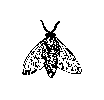
\includegraphics{fly}
\caption{A sample black and white graphic.}
\end{figure}

\begin{figure}
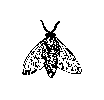
\includegraphics[height=1in, width=1in]{fly}
\caption{A sample black and white graphic
that has been resized with the \texttt{includegraphics} command.}
\end{figure}


As was the case with tables, you may want a figure that spans two
columns.  To do this, and still to ensure proper ``floating''
placement of tables, use the environment \textbf{figure*} to enclose
the figure and its caption.  And don't forget to end the environment
with \textbf{figure*}, not \textbf{figure}!

\begin{figure*}
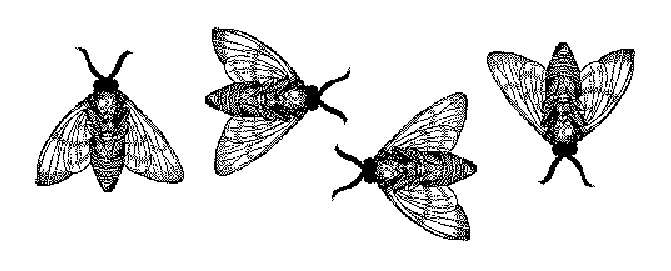
\includegraphics{flies}
\caption{A sample black and white graphic
that needs to span two columns of text.}
\end{figure*}


\begin{figure}
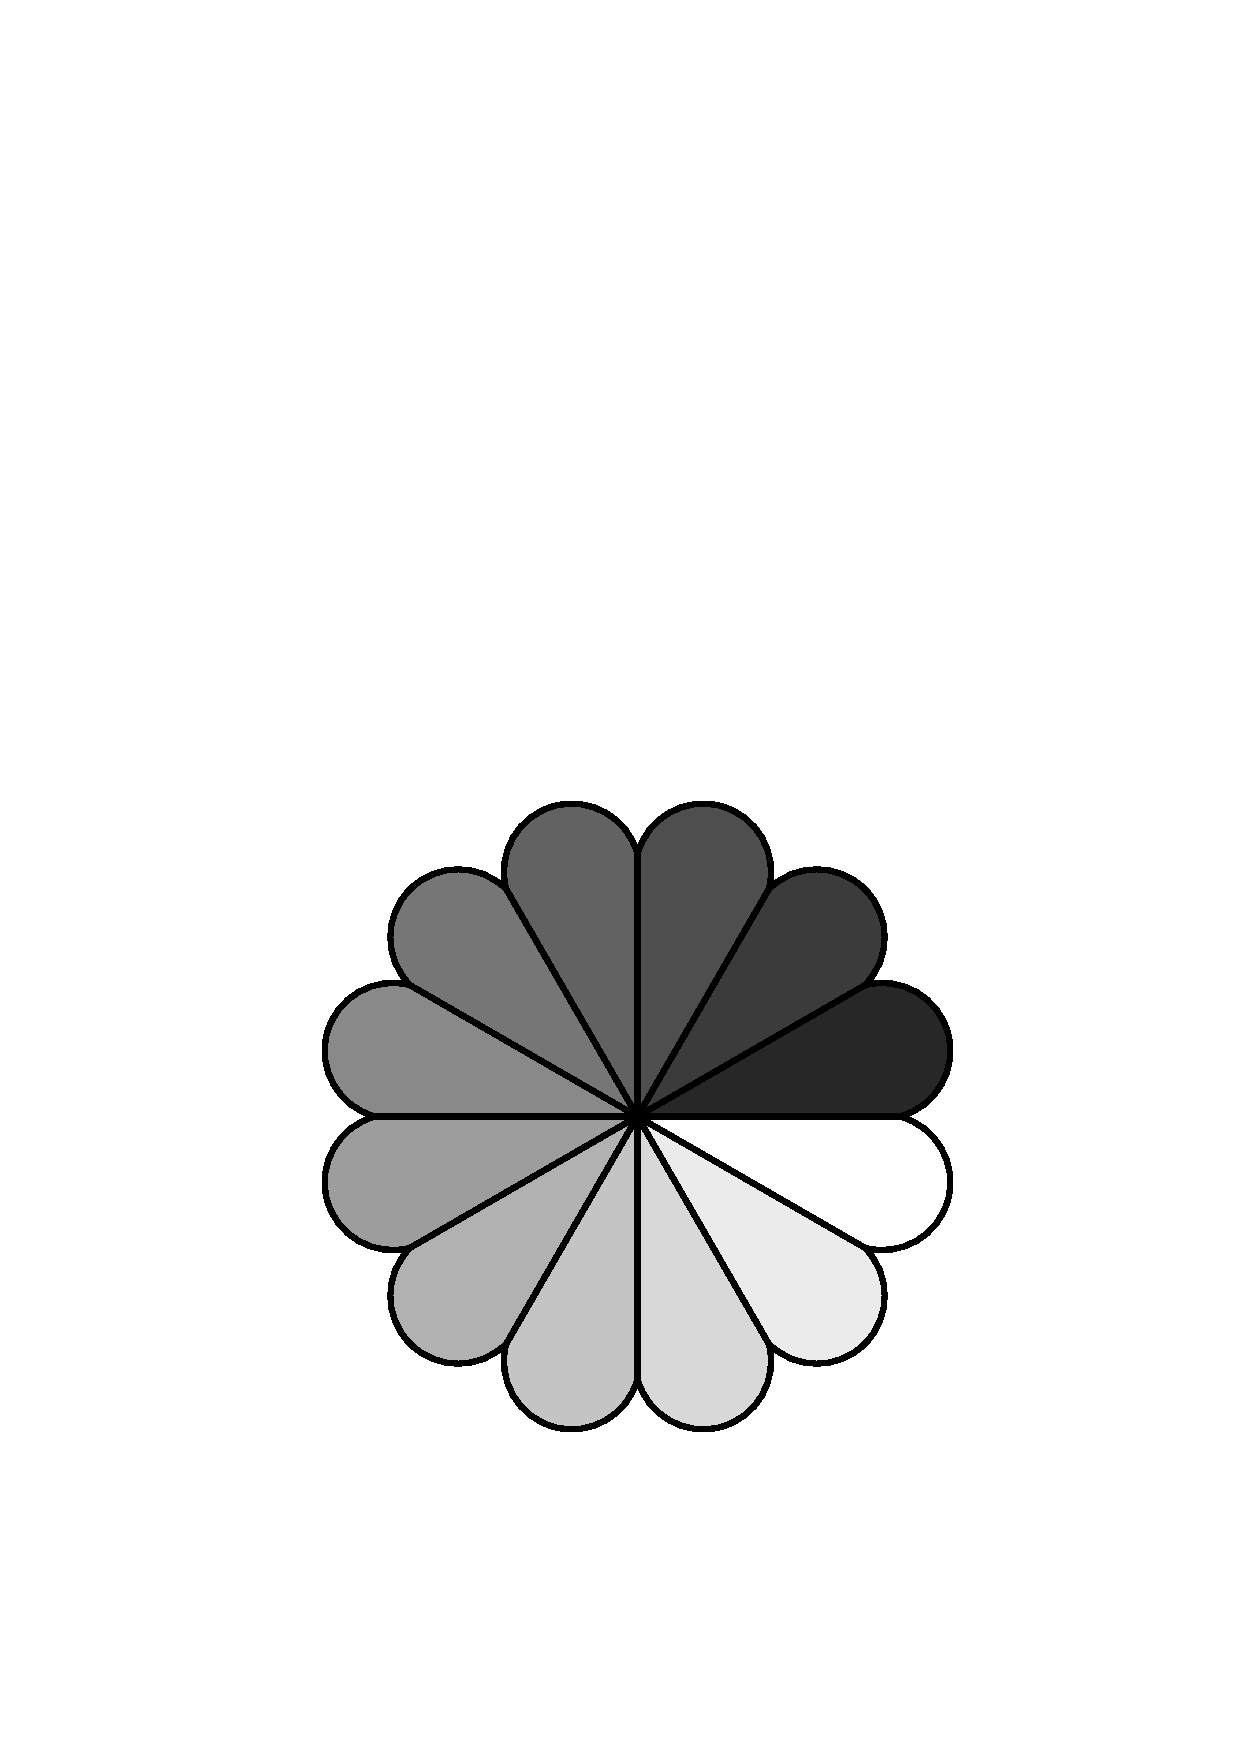
\includegraphics[height=1in, width=1in]{rosette}
\caption{A sample black and white graphic that has
been resized with the \texttt{includegraphics} command.}
\end{figure}

\subsection{Theorem-like Constructs}

Other common constructs that may occur in your article are the forms
for logical constructs like theorems, axioms, corollaries and proofs.
ACM uses two types of these constructs:  theorem-like and
definition-like.

Here is a theorem:
\begin{theorem}
  Let $f$ be continuous on $[a,b]$.  If $G$ is
  an antiderivative for $f$ on $[a,b]$, then
  \begin{displaymath}
    \int^b_af(t)\,dt = G(b) - G(a).
  \end{displaymath}
\end{theorem}

Here is a definition:
\begin{definition}
  If $z$ is irrational, then by $e^z$ we mean the
  unique number that has
  logarithm $z$:
  \begin{displaymath}
    \log e^z = z.
  \end{displaymath}
\end{definition}

The pre-defined theorem-like constructs are \textbf{theorem},
\textbf{conjecture}, \textbf{proposition}, \textbf{lemma} and
\textbf{corollary}.  The pre-defined de\-fi\-ni\-ti\-on-like constructs are
\textbf{example} and \textbf{definition}.  You can add your own
constructs using the \textsl{amsthm} interface~\cite{Amsthm15}.  The
styles used in the \verb|\theoremstyle| command are \textbf{acmplain}
and \textbf{acmdefinition}.

Another construct is \textbf{proof}, for example,

\begin{proof}
  Suppose on the contrary there exists a real number $L$ such that
  \begin{displaymath}
    \lim_{x\rightarrow\infty} \frac{f(x)}{g(x)} = L.
  \end{displaymath}
  Then
  \begin{displaymath}
    l=\lim_{x\rightarrow c} f(x)
    = \lim_{x\rightarrow c}
    \left[ g{x} \cdot \frac{f(x)}{g(x)} \right ]
    = \lim_{x\rightarrow c} g(x) \cdot \lim_{x\rightarrow c}
    \frac{f(x)}{g(x)} = 0\cdot L = 0,
  \end{displaymath}
  which contradicts our assumption that $l\neq 0$.
\end{proof}

\section{Conclusions}
This paragraph will end the body of this sample document.
Remember that you might still have Acknowledgments or
Appendices; brief samples of these
follow.  There is still the Bibliography to deal with; and
we will make a disclaimer about that here: with the exception
of the reference to the \LaTeX\ book, the citations in
this paper are to articles which have nothing to
do with the present subject and are used as
examples only.
%\end{document}  % This is where a 'short' article might terminate



\appendix
%Appendix A
\section{Headings in Appendices}
The rules about hierarchical headings discussed above for
the body of the article are different in the appendices.
In the \textbf{appendix} environment, the command
\textbf{section} is used to
indicate the start of each Appendix, with alphabetic order
designation (i.e., the first is A, the second B, etc.) and
a title (if you include one).  So, if you need
hierarchical structure
\textit{within} an Appendix, start with \textbf{subsection} as the
highest level. Here is an outline of the body of this
document in Appendix-appropriate form:
\subsection{Introduction}
\subsection{The Body of the Paper}
\subsubsection{Type Changes and  Special Characters}
\subsubsection{Math Equations}
\paragraph{Inline (In-text) Equations}
\paragraph{Display Equations}
\subsubsection{Citations}
\subsubsection{Tables}
\subsubsection{Figures}
\subsubsection{Theorem-like Constructs}
\subsubsection*{A Caveat for the \TeX\ Expert}
\subsection{Conclusions}
\subsection{References}
Generated by bibtex from your \texttt{.bib} file.  Run latex,
then bibtex, then latex twice (to resolve references)
to create the \texttt{.bbl} file.  Insert that \texttt{.bbl}
file into the \texttt{.tex} source file and comment out
the command \texttt{{\char'134}thebibliography}.
% This next section command marks the start of
% Appendix B, and does not continue the present hierarchy
\section{More Help for the Hardy}

Of course, reading the source code is always useful.  The file
\path{acmart.pdf} contains both the user guide and the commented
code.

\begin{acks}
  The authors would like to thank Dr. Yuhua Li for providing the
  matlab code of  the \textit{BEPS} method. 

  The authors would also like to thank the anonymous referees for
  their valuable comments and helpful suggestions. The work is
  supported by the \grantsponsor{GS501100001809}{National Natural
    Science Foundation of
    China}{http://dx.doi.org/10.13039/501100001809} under Grant
  No.:~\grantnum{GS501100001809}{61273304}
  and~\grantnum[http://www.nnsf.cn/youngscientsts]{GS501100001809}{Young
    Scientsts' Support Program}.

\end{acks}


\bibliographystyle{ACM-Reference-Format}
\bibliography{sigproc,dissertation} 

\end{document}
